\section{Dimensions}
\label{sec:forward_dimensions}
{\small
\begin{center}
\begin{longtable}{| p{1.2in} || p{1.0in} | p{4.0in} |}
	\hline 
	{\bf Name} & {\bf Units} & {\bf Description} \endfirsthead
	\hline 
	{\bf Name} & {\bf Units} & {\bf Description} (Continued) \endhead
	\hline 
	\hline 
	nCells & $unitless$ & The number of polygons in the primary grid. \\ 
	\hline
	nEdges & $unitless$ & The number of edge midpoints in either the primary or dual grid. \\ 
	\hline
	maxEdges & $unitless$ & The largest number of edges any polygon within the grid has. \\ 
	\hline
	maxEdges2 & $unitless$ & Two times the largest number of edges any polygon within the grid has. \\ 
	\hline
	nAdvectionCells & $unitless$ & The largest number of advection cells for any edge. \\ 
	\hline
	nVertices & $unitless$ & The total number of cells in the dual grid. Also the number of corners in the primary grid. \\ 
	\hline
	TWO & $unitless$ & The number two as a dimension. \\ 
	\hline
	R3 & $unitless$ & The number three as a dimension. \\ 
	\hline
	SIX & $unitless$ & The number six as a dimension. \\ 
	\hline
	FIFTEEN & $unitless$ & The number 15 as a dimension. \\ 
	\hline
	TWENTYONE & $unitless$ & The number 21 as a dimension. \\ 
	\hline
	vertexDegree & $unitless$ & The number of cells or edges touching each vertex. \\ 
	\hline
	nVertLevels & $unitless$ & The number of levels in the vertical direction. All vertical levels share the same horizontal locations. \\ 
	\hline
	nVertLevelsP1 & $unitless$ & The number of interfaces in the vertical direction. \\ 
	\hline
	nZonalMeanBins & $unitless$ & Maximum number of bins for zonal mean. \\ 
	\hline
	nZonalMeanBinsP1 & $unitless$ & Maximum number of bins for zonal mean, plus one. \\ 
	\hline
\end{longtable}
\end{center}
}
\section[Namelist options]{\hyperref[chap:namelist_sections]{Namelist options}}
\label{sec:forward_namelist_tables}
Embedded links point to more detailed namelist information in the appendix.
\subsection[time\_management]{time\_management}
\label{subsec:forward_nm_tab_time_management}
General time management is handled by the time\_management namelist record.
Included options handle time-related parts of MPAS, such as the calendar and if the simulation is a restart or not.

Users should use this record to specify the beginning time of the simulation,
and either the duration or the end of the simulation. Only the end or the
duration need to be specified as the other is derived within MPAS from the
beginning time and other specified one.

{\bf TBA: If both duration and stop are specified, then what happens?)}

\vspace{0.5in}
{\small
\begin{center}
\begin{longtable}{| p{2.0in} || p{4.0in} |}
	\hline
	{\bf Name} & {\bf Description} \endfirsthead
	\hline 
	{\bf Name} & {\bf Description} (Continued) \endhead
	\hline
	\hline
	\hyperref[sec:nm_sec_config_do_restart]{config\_do\_restart} & Determines if the initial conditions should be read from a restart file, or an input file. \\
	\hline
	\hyperref[sec:nm_sec_config_restart_timestamp_name]{config\_restart\_timestamp\_name} & Path to the filename for restart timestamps to be read and written from. \\
	\hline
	\hyperref[sec:nm_sec_config_start_time]{config\_start\_time} & Timestamp describing the initial time of the simulation. If it is set to 'file', the initial time is read from restart\_timestamp. \\
	\hline
	\hyperref[sec:nm_sec_config_stop_time]{config\_stop\_time} & Timestamp descriping the final time of the simulation. If it is set to 'none' the final time is determined from config\_start\_time and config\_run\_duration. \\
	\hline
	\hyperref[sec:nm_sec_config_run_duration]{config\_run\_duration} & Timestamp describing the length of the simulation. If it is set to 'none' the duration is determined from config\_start\_time and config\_stop\_time. config\_run\_duration overrides inconsistent values of config\_stop\_time. \\
	\hline
	\hyperref[sec:nm_sec_config_calendar_type]{config\_calendar\_type} & Selection of the type of calendar that should be used in the simulation. \\
	\hline
\end{longtable}
\end{center}
}
\subsection[io]{io}
\label{subsec:forward_nm_tab_io}
The io namelist record provides options for modifications to the I/O system of
MPAS. These include frequency, file name, and parallelization options.

\vspace{0.5in}
{\small
\begin{center}
\begin{longtable}{| p{2.0in} || p{4.0in} |}
	\hline
	{\bf Name} & {\bf Description} \endfirsthead
	\hline 
	{\bf Name} & {\bf Description} (Continued) \endhead
	\hline
	\hline
	\hyperref[sec:nm_sec_config_stats_interval]{config\_stats\_interval} & Timestamp determining how often a global statistics files should be written. \\
	\hline
	\hyperref[sec:nm_sec_config_write_stats_on_startup]{config\_write\_stats\_on\_startup} & Logical flag determining if statistics files should be written prior to the first time step. \\
	\hline
	\hyperref[sec:nm_sec_config_write_output_on_startup]{config\_write\_output\_on\_startu-}\hyperref[sec:nm_sec_config_write_output_on_startup]{p}& Logical flag determining if an output file should be written prior to the first time step. \\
	\hline
	\hyperref[sec:nm_sec_config_pio_num_iotasks]{config\_pio\_num\_iotasks} & Integer specifying how many IO tasks should be used within the PIO library. A value of 0 causes all MPI tasks to also be IO tasks. IO tasks are requried to write contiguous blocks of data to a file. \\
	\hline
	\hyperref[sec:nm_sec_config_pio_stride]{config\_pio\_stride} & Integer specifying the stride of each IO task. \\
	\hline
\end{longtable}
\end{center}
}
\subsection[time\_integration]{time\_integration}
\label{subsec:forward_nm_tab_time_integration}
The time integration namelist controls parameters that pertain to all time-stepping methods.  At present, Forward Euler is the only time integration method implemented.

\vspace{0.5in}
{\small
\begin{center}
\begin{longtable}{| p{2.0in} || p{4.0in} |}
	\hline
	{\bf Name} & {\bf Description} \endfirsthead
	\hline 
	{\bf Name} & {\bf Description} (Continued) \endhead
	\hline
	\hline
	\hyperref[sec:nm_sec_config_dt]{config\_dt} & Length of model time-step. \\
	\hline
	\hyperref[sec:nm_sec_config_time_integrator]{config\_time\_integrator} & Time integration method. \\
	\hline
\end{longtable}
\end{center}
}
\subsection[ALE\_vertical\_grid]{ALE\_vertical\_grid}
\label{subsec:forward_nm_tab_ALE_vertical_grid}
The MPAS-Ocean vertical grid is structured arbitrary Lagrangian-Eulerian (ALE).   ALE provides a great deal of freedom in the choice of vertical coordinate: when fully Eulerian, MPAS-Ocean is a z-level model with fixed thicknesses; when fully Lagrangian, there is no vertical transport between layers, and layers expand and contract like an isopycnal ocean model.  In between are many additional options, such as z-star where layers expand in proportion to the sea surface height, and sigma, where coordinates are terrain-following.

MPAS-Ocean employs the continuity equation,
\begin{eqnarray}
\label{ocean:continuity thickness}
\frac{\partial h_{k}}{\partial t} + D_k + w^t_k - w^t_{k+1} =0
\end{eqnarray}
for the ALE formulation, where variables are defined in Table \ref{oceanTable:ALE_variables}.  The ALE algorithm is as follows:
\begin{enumerate}
\item ALE step: Compute desired thickness for the new time,
\begin{eqnarray}
\label{ocean:desired thickness}
h_k^{ALE} = h_k^{rest} + h_k^{SSH} + h_k^{hf} + h_k^{min}
\end{eqnarray}
\item ALE step: Solve for vertical transport $w^t$ from (\ref{ocean:continuity thickness}),
\begin{eqnarray}
\label{ocean:vert tranport}
w^t_k = w^t_{k+1} - D_k - \frac{h^{ALE}_k - h^n_k}{\Delta t}
\end{eqnarray}
\item Solve for new thickness, $h_{k}^{n+1}$, using the continuity equation (\ref{ocean:continuity thickness}) within the time integration routine.
\end{enumerate}
The redundancy in steps 2 and 3 are intentional, so that step 2 is isolated within the ALE subroutine, and step 3 is solved in the timestepping subroutine in the identical manner as the tracer equation (\ref{ocean:tracer}).

The desired ALE thickness includes contributions from four terms (\ref{ocean:desired thickness}):
\begin{enumerate}
\item {\bf Resting thickness}, $h^{rest}$, is the layer thickness when the ocean is at rest, i.e. without SSH or internal perturbations.  For z-type coordinates, the resting thickness is constant in each horizontal layer.
\item {\bf SSH alteration}, $h^{SSH}$, alters layer thicknesses so that they change in proportion to the sea surface height (SSH),
\begin{eqnarray}
\label{ocean:h ssh}
   h_k^{SSH} =  \zeta \frac{W_k h^{rest}_k}{\sum_{k'=1}^{kmax}W_{k'}h^{rest}_{k'}}
\end{eqnarray}
The weights $W_k$ determine how SSH oscillations are distributed amongst the layers, as described in Table \ref{oceanTable:vertical coordinates}.
\item {\bf High-frequency thickness}, $h^{hf}$, allows high-frequency thickness oscillations, such as internal gravity waves, to be treated in a Lagrangian manner.  This is the ``z-tilde'' scheme of \citet{Leclair_Madec11om} described in the next section.
\item {\bf Minimum thickness alteration}, $h^{min}$, is the change in thickness required to enforce the minimum thickness in each cell.  When a cell is too thin, $h^{min}$ is positive, while nearby cells in the vertical incur a corresponding negative $h^{min}$ to conserve volume in the column.
\end{enumerate}
Of the four terms, resting thickness is always positive, while the others are small alterations about zero.  Summing a column,
\begin{eqnarray}
\sum_{k=1}^{kmax} h_k^{ALE} &=& \sum_{k=1}^{kmax} h_k^{rest} + \sum_{k=1}^{kmax}h_k^{SSH} + \sum_{k=1}^{kmax}h_k^{hf} + \sum_{k=1}^{kmax}h_k^{min} 
\nonumber \\
&=& H + \zeta + 0 + 0.
\nonumber
\end{eqnarray}
Thus the first two terms are always included so that the column thickness sums to $H+\zeta$, while the second two terms are optional and may be turned on with flags.

In order to assist users in choosing the correct settings, we provide a description of traditional vertical coordinate names in Table \ref{oceanTable:vertical coordinates}.
The vertical coordinate type also depends upon the set-up of the layerThickness variable in the initial condition file.  For all Z-type vertical coordinates, initial layer thicknesses are horizontally constant.  For sigma coordinates, layers are terrain-following and all layers are employed.  In this case, the user may still choose amongst the flags in SSH may be distributed through the column just like with z-type models in Table \ref{oceanTable:vertical coordinates}.

In order to run an isopycnal configuration, use config\_vert\_coord\_movement='impermeable\_interfaces' and set initial temperature and salinity to be constant within each layer.  All vertical tracer diffusion must be off so that the density in each layer remains constant.  For an isopycnal set-up, the equation of state is still called at each timestep, so a linear equation of state is recommended to avoid depth-dependancy of the density.  The user may choose a Montgomery Potential (\ref{ocean:Montgomery Potential}) or standard pressure gradient (\ref{ocean:grad p}); Montgomery Potential is a more common choice for isopycnal configurations, but both are tested and functional.  MPAS-Ocean does not support massless layers at this time, so isopycnal vertical coordinates may only be used for idealized domains.

\begin{table}[ht] 
\caption{Vertical coordinate settings for traditional names.}
\vspace{0.5cm} \centering 
\begin{tabular}{c c c c c c} 
\hline\hline flag name &  {\bf Z-Level} & {\bf Z-star} & {\bf weighted Z-star} &  {\bf isopycnal}  \\
\hline 
config\_vert\_ & 'fixed' & 'uniform\_stretching' & 'user\_specified' & 'impermeable\_ \\
coord\_movement & & & & interfaces'
\\
weights & $W_k =\left\{ \begin{array}{c} 1\; k=1\\ 0\; k>1 \end{array}\right.$ & $W_k=1\;\;\forall\;\;k$ & input file & not applicable \\
\hline 
\end{tabular} \label{oceanTable:vertical coordinates} 
\end{table}

\begin{table}[h!t] 
\caption{Variables used in ALE equation sets.  Column 3 shows the native horizontal grid location.  A subscript $k$ indicates indicates the layer index.  The $\nabla$ indicates a horizontal gradient within a single layer.} 
\vspace{0.5cm} \centering 
\begin{tabular}{c c c c } 
\hline\hline symbol &  name & grid &  notes  \\
\hline 
$D$  & thickness-weighted divergence & cell & $D_k = \nabla \cdot  \left( h_k {\bf u}_k \right)$  \\ 
${\bar D}$ & barotropic divergence & cell & ${\overline D} = \sum\limits_{k=1}^{kmax} D_k$  \\ 
$D'$  & baroclinic divergence & cell & $D'_k = D_k-\frac{h_k}{H}{\bar D}$  \\ 
$D^{lf}$  & low-frequency divergence & cell & see (\ref{ocean:Dlf})  \\ 
$D^{hf}$  & high-frequency divergence & cell & $D^{hf}_k = D'_k - D^{lf}_k$  \\ 
$h$  & layer thickness & cell &   \\ 
$h^{ALE}$  & desired ALE thickness & cell & see (\ref{ocean:desired thickness})  \\ 
$h^{rest}$  & resting thickness & cell &   \\ 
$h^{SSH}$  & SSH thickness alteration & cell & see (\ref{ocean:h ssh})  \\ 
$h^{hf}$  & high-freq. thickness alteration & cell &   see (\ref{ocean:hhf})  \\ 
$h^{min}$  & minimum thickness alteration & cell &   \\ 
$H$  & total resting thickness & cell & $H= \sum\limits_{k=1}^{kmax} h_k^{rest}$  \\ 
${\bf u}$  & velocity & edge &   \\ 
$w^t$ & vertical transport & cell  & top of layer in vertical \\
$W$  & SSH thickness weights & cell &   \\ 
$\tau_{Dlf}$  & frequency filter time scale & constant &   \\ 
$\tau_{hhf}$  & restoring time scale for $h^{hf}$ & constant &   \\ 
$\kappa_{hhf}$  & $h^{hf}$ diffusion & constant &   \\ 
$\zeta$  & sea surface height & cell &  $\zeta= \sum\limits_{k=1}^{kmax} h_k^{rest} - H$  \\ 
\hline 
\end{tabular} \label{oceanTable:ALE_variables} 
\end{table}


\vspace{0.5in}
{\small
\begin{center}
\begin{longtable}{| p{2.0in} || p{4.0in} |}
	\hline
	{\bf Name} & {\bf Description} \endfirsthead
	\hline 
	{\bf Name} & {\bf Description} (Continued) \endhead
	\hline
	\hline
	\hyperref[sec:nm_sec_config_vert_coord_movement]{config\_vert\_coord\_movement} &  Determines the vertical coordinate movement type. 'uniform\_stretching' distributes SSH perturbations through all vertical levels (z-star vertical coordinate); 'fixed' places them all in the top level (z-level vertical coordinate); 'user\_specified' allows the input file to determine the distribution using the variable vertCoordMovementWeights (weighted z-star vertical coordinate); and 'impermeable\_interfaces' makes the vertical transport between layers zero, i.e.  $w^t=0$  (idealized isopycnal). \\
	\hline
	\hyperref[sec:nm_sec_config_use_min_max_thickness]{config\_use\_min\_max\_thickness} & If true, a minimum and maximum thicknesses are enforced to prevent massless and very thick layers. \\
	\hline
	\hyperref[sec:nm_sec_config_min_thickness]{config\_min\_thickness} & Minimum thickness allowed. \\
	\hline
	\hyperref[sec:nm_sec_config_max_thickness_factor]{config\_max\_thickness\_factor} &  Maximum thickness allowed. This is a factor times the resting thickness, i.e., maximum thickness = config\_max\_thickness\_factor* $h^{rest}$ . \\
	\hline
	\hyperref[sec:nm_sec_config_set_restingThickness_to_IC]{config\_set\_restingThickness\_t-}\hyperref[sec:nm_sec_config_set_restingThickness_to_IC]{o\_IC}& If true, set restingThickness to be the same as layerThickness upon start-up. This only occurs when config\_do\_restart is false, i.e. on an initial run. \\
	\hline
	\hyperref[sec:nm_sec_config_dzdk_positive]{config\_dzdk\_positive} & Determines if the positive Z axis is aligned with the positive K index direction. \\
	\hline
\end{longtable}
\end{center}
}
\subsection[ALE\_frequency\_filtered\_thickness]{ALE\_frequency\_filtered\_thickness}
\label{subsec:forward_nm_tab_ALE_frequency_filtered_thickness}
The high-frequency thickness alteration, $h^{hf}$, in (\ref{ocean:\mode_desired thickness}) allows the thicknesses to oscillate so that high-frequency motions, such as internal gravity waves, are treated in a Lagrangian manner.  Low-freqency motions, such as seasonal changes or slow motions of water masses, are treated in an Eulerian manner.  This is the ``z-tilde'' scheme of \citet{Leclair_Madec11om}, which generally reduces spurious vertical mixing and preserves water mass properties.  Two additional prognostic equations are solved when config\_use\_freq\_filtered\_thickness is true,
\begin{eqnarray}
\label{ocean:\mode_Dlf}
 & \displaystyle
  \frac{\partial D^{lf}_k}{\partial t} = - \frac{2\pi}{\tau_{Dlf}} \left( D^{lf}_k - D'_k \right), 
\\ & \displaystyle
\label{ocean:\mode_hhf}
\frac{\partial h^{hf}_k}{\partial t} =  - D^{hf}_k - \frac{2\pi}{\tau_{hhf}} h^{hf}_k + \nabla_h\cdot \left( \kappa_{hhf} \nabla_h h^{hf}_k \right) 
\end{eqnarray}
where $\tau_{Dlf}$ is the filter timescale and other variables are defined in Table \ref{oceanTable:\mode_ALE_variables}.  This may be used in addition to any of the z-type or sigma-type vertical coordinates in Table \ref{oceanTable:\mode_vertical coordinates}.  Some combination of thickness restoring and diffusion are recommended to avoid long-term drift of $h^{hf}$ away from zero.




\vspace{0.5in}
{\small
\begin{center}
\begin{longtable}{| p{2.0in} || p{4.0in} |}
	\hline
	{\bf Name} & {\bf Description} \endfirsthead
	\hline 
	{\bf Name} & {\bf Description} (Continued) \endhead
	\hline
	\hline
	\hyperref[sec:nm_sec_config_use_freq_filtered_thickness]{config\_use\_freq\_filtered\_thickn-}\hyperref[sec:nm_sec_config_use_freq_filtered_thickness]{ess}&  If true,  $h^{hf}$  is included in the desired ALE thickness, and the prognostic equations for  $D^{lf}$  and  $h^{hf}$  are integrated in the code. \\
	\hline
	\hyperref[sec:nm_sec_config_thickness_filter_timescale]{config\_thickness\_filter\_timescal-}\hyperref[sec:nm_sec_config_thickness_filter_timescale]{e}&  Filter time scale for the low-frequency baroclinic divergence,  $\tau_{Dlf}$ . \\
	\hline
	\hyperref[sec:nm_sec_config_use_highFreqThick_restore]{config\_use\_highFreqThick\_rest-}\hyperref[sec:nm_sec_config_use_highFreqThick_restore]{ore}&  If true, the high frequency thickness prognostic equation ( $h^{hf}$ ) includes term 2 on the RHS, the restoring term.  The high frequency thickness is restored to zero with time scale  $\tau_{hhf}$ . \\
	\hline
	\hyperref[sec:nm_sec_config_highFreqThick_restore_time]{config\_highFreqThick\_restore\_-}\hyperref[sec:nm_sec_config_highFreqThick_restore_time]{time}&  Restoring time scale for high-frequency thickness,  $\tau_{hhf}$ . \\
	\hline
	\hyperref[sec:nm_sec_config_use_highFreqThick_del2]{config\_use\_highFreqThick\_del2} &  If true, high frequency thickness prognostic equation ( $h^{hf}$ ) includes term 3 on the RHS, the diffusion term. \\
	\hline
	\hyperref[sec:nm_sec_config_highFreqThick_del2]{config\_highFreqThick\_del2} &  Horizonal high frequency thickness diffusion,  $\kappa_{hhf}$ . \\
	\hline
\end{longtable}
\end{center}
}
\subsection[partial\_bottom\_cells]{partial\_bottom\_cells}
\label{subsec:forward_nm_tab_partial_bottom_cells}
\documentclass[11pt]{report}

\usepackage{epsf,amsmath,amsfonts}
\usepackage{graphicx}

\setlength{\textwidth}{6.5in}
\setlength{\oddsidemargin}{0in}
\setlength{\evensidemargin}{0in}
\setlength{\textheight}{8.5in}
\setlength{\topmargin}{0in}

\begin{document}

\title{
Requirements and Design\\
Partial Bottom Cells}
\author{MPAS Development Team}

\maketitle
\tableofcontents

%-----------------------------------------------------------------------

\chapter{Summary}

Partial bottom cells (PBCs) allow bottom topography to be represented more realistically.  Currently, MPAS-Ocean only suports full ocean cells, so the bottom depth of a column is restricted to the depth of each vertical cell interface.  With partial bottom cells, the bottom depth may take on any value.  This is still a z-level-type formulation, where cells that are fully below the bottom depth are considered land cells.  The PBC formulation will work with z-level, z-star, and z-tilde formulations.

%figure template
%\begin{figure}
%  \center{\includegraphics[width=14cm]{./Figure1.pdf}}
%  \caption{A graphical representation of the discrete boundary.}
%  \label{Figure1}
%\end{figure} 

%-----------------------------------------------------------------------

\chapter{Requirements}

\section{Requirement: initial conditions with consistant variables}
Date last modified: 2012/10/15 \\
Contributors: Mark Petersen \\

The following variables must be consistent upon starting a new simulation with mpas-ocean: bottomDepth, maxLevelCell, thickness $h$, location of initial tracers in bottom cell.

\section{Requirement: horizontal advection}
Date last modified: 2012/08/01 \\
Contributors: Mark Petersen \\

Horizontal advection must take place through a thickness that accounts for the partial bottom cell at the bottom of the column.

\section{Requirement: pressure gradient}
Date last modified: 2012/08/01 \\
Contributors: Mark Petersen \\

Pressure gradients must not contain spurious effects due to the partial bottom cells.



%-----------------------------------------------------------------------

\chapter{Algorithmic Formulations}

\section{Design Solution: initial conditions with consistant variables}

Date last modified: 2012/10/15 \\
Contributors: Mark Petersen \\

The thickness variable {\tt h(k,iCell,iStep)} will continue to be the actual thickness of fluid in the cell.  
A new variable, {\tt bottomDepth(iCell)}, is the depth below the average sea surface height ($z=0$) in each cell, and is a positive number.    The variable {\tt maxLevelCell(iCell)} is an integer of the deepest active (water-filled) cell, and {\tt refBottomDepth(k)} is the depth of the bottom of each cell in z-level coordinates.  Note that depth variables are positive, $z$ variables are negative and decrease with greater depths, and the $k$ index increases with greater depth.

In generating the initial conditions (IC), the following steps are taken:
\begin{enumerate}
\item An additional parameter, {\tt max\_partial\_bottom\_cell}, may be set between zero and one, with default .95, in the initial condition generation.  Then {\tt bottomDepth} must be altered so that a partial bottom cell has a maximum of (say) 95\% land.  This parameter may be adjusted after testing. 
\item The thickness {\tt h} at {\tt k=maxLevelCell} is reduced to take into account the thickness removed by the partial bottom cell.
\item Initial tracer values in the bottom cell are interpolated to the center of the pbc, rather than the center of the full cell.
\item Check that {\tt bottomDepth} corresponds to {\tt maxLevelCell} (because they are redundant):\\
when {\tt k=maxLevelCell(iCell)}:\\
{\tt refBottomDepth(k)<bottomDepth(iCell)< refBottomDepth(k-1)}
\end{enumerate}

The ICs could be altered in basin.F or upon start-up with mpas.  We chose to alter the ICs in mpas to reduce the number and IC files and the complexity of IC generation.  The initial netcdf file (ocean.nc, produced by basin), include a realistic
 bottomDepth variable and thickness and tracer variables for full thickness cells.

Upon start-up with {\tt config\_do\_restart = .false.}, ICs are altered as described above.  An additional flag is used as follows:
\begin{itemize}
\item If running with pbcs, set {\tt config\_alter\_ICs\_for\_pbc='zlevel\_pbcs\_on'}. Then thin pbc cells
   will be changed, and thickness and tracers will be altered to match the pbcs (steps 1-3, above).
\item If running without pbcs, set {\tt config\_alter\_ICs\_for\_pbc='zlevel\_pbcs\_off'}. Then 
   bottomDepth will be altered so it is full cells everywhere.
   If your input file does not include bottomDepth, the false option will
   initialize bottomDepth correctly for a non-pbc run.
\item Set {\tt config\_alter\_ICs\_for\_pbc='no'} for isopycnal or sigma coordinates.
\end{itemize}

Consistency between {\tt bottomDepth} and {\tt maxLevelCell} is verified afterwards if {\tt config\_check\_zlevel\_consistency=.true.}


\section{Design Solution: horizontal advection}
Date last modified: 2012/08/01 \\
Contributors: Mark Petersen \\

{\bf Option 1: Do nothing (this option was chosen)}\\

If nothing is changed in the current code, {\tt h\_edge} is computed from from the thickness of nearby cells, regardless of PBCs in the bottom layer.  This is a clean and simple solution, but if PBCs are very thin, a cell could be evacuated of water.\\

{\bf Option 2: h\_edge is limited by minimum depth of neighboring cells}\\

In POP, the thickness of a U-cell is the minimum of the four surrounding T-Cells.  Likewise in MPAS-Ocean, one could compute the edge thickness using the minimum bottom depth of the two surrounding cells.  For the computation of {\tt h\_edge} using higher order advection methods, this will require further thought.

\section{Design Solution: pressure gradient}
Date last modified: 2012/08/01 \\
Contributors: Mark Petersen \\

{\bf Option 1: Do nothing (this option was chosen)}\\

MPAS-Ocean currently has two terms related to the pressure gradient,
\begin{equation}
- \frac{1}{\rho_0}\nabla p_k  - \frac{\rho g}{\rho_0}\nabla z^{mid}_k.
\end{equation}
where the gradient of $z^{mid}$ makes up pressure differences due to tilted levels.  However, in a stratified ocean, pressure gradient errors occur when the tilting of levels is large.  In a z-star system without PBCs, these perturbations are limited by the ratio of sea surface height to total depth, so only a few percent.  With the inclusion of PBCs, $z^{mid}$ could vary from one gridcell to the next by half the layer thickness.\\

{\bf Option 2: Interpolate T \& S to center of bottom cell for pressure computation}\\

If the pressure gradient errors are deemed to be too large, one could extrapolate the temperature and salinity values to the mid-depth of the bottom cell, and compute density and pressure at that location.  This will require a special case when {\tt k=maxLevelCell}.  There will need to be an extra case in the computation of $\nabla z^{mid}$ as well, so that $z^{mid}$ at the bottom cell is at the cell center.


%-----------------------------------------------------------------------

\chapter{Design and Implementation}

\section{Implementation: consistency between thickness and partial bottom cell variables}
Date last modified: 2012/08/01 \\
Contributors: Mark Petersen \\


\section{Implementation: horizontal advection}
Date last modified: 2012/08/01 \\
Contributors: Mark Petersen \\


\section{Implementation: pressure gradient}
Date last modified: 2012/08/01 \\
Contributors: Mark Petersen \\


%-----------------------------------------------------------------------

\chapter{Testing}

\section{Testing and Validation: Partial bottom cells}
Date last modified: 2012/08/01 \\
Contributors: Mark Petersen \\

Use the test problem, already in the repository, following Ilicak ea 2012 overflow test case (\#4).


%-----------------------------------------------------------------------

\end{document}

\vspace{0.5in}
{\small
\begin{center}
\begin{longtable}{| p{2.0in} || p{4.0in} |}
	\hline
	{\bf Name} & {\bf Description} \endfirsthead
	\hline 
	{\bf Name} & {\bf Description} (Continued) \endhead
	\hline
	\hline
	\hyperref[sec:nm_sec_config_alter_ICs_for_pbcs]{config\_alter\_ICs\_for\_pbcs} & If true, initial conditions are altered according to the config\_pbc\_alteration\_type flag. The alteration of layer thickness only occurs when config\_do\_restart is false, i.e. on an initial run. \\
	\hline
	\hyperref[sec:nm_sec_config_pbc_alteration_type]{config\_pbc\_alteration\_type} & Determines the method of initial condition alteration for partial bottom cells. 'partial\_cell' alters layerThickness, interpolates all tracers in the bottom cell based on the bottomDepth variable, and alters bottomDepth to enforce the minimum pbc fraction. 'full\_cell' alters bottomDepth to have full cells everywhere, based on the refBottomDepth variable. \\
	\hline
	\hyperref[sec:nm_sec_config_min_pbc_fraction]{config\_min\_pbc\_fraction} & Determines the minimum fraction of a cell altering the initial conditions can create. The alteration of layer thickness only occurs when config\_do\_restart is false, i.e. on an initial run. \\
	\hline
	\hyperref[sec:nm_sec_config_check_ssh_consistency]{config\_check\_ssh\_consistency} &  Enables a check to determine if the SSH is within 2m of the surface.  See equation for  $\zeta_i$ . \\
	\hline
\end{longtable}
\end{center}
}
\subsection[decomposition]{decomposition}
\label{subsec:forward_nm_tab_decomposition}
MPAS handles decomposing all variables into computational blocks. The
decomposition used needs to be specified at run time and is computed by an
external tool (e.g. metis). Additionally, MPAS supports multiple computational
blocks per MPI process, and the user may specify an additional decomposition
file which can specify the assignment of blocks to MPI processes. Run-time
parameters that control the run-time decomposition used are specified within
the decomposition namelist record.


\vspace{0.5in}
{\small
\begin{center}
\begin{longtable}{| p{2.0in} || p{4.0in} |}
	\hline
	{\bf Name} & {\bf Description} \endfirsthead
	\hline 
	{\bf Name} & {\bf Description} (Continued) \endhead
	\hline
	\hline
	\hyperref[sec:nm_sec_config_num_halos]{config\_num\_halos} & Determines the number of halo cells extending from a blocks owned cells (Called the 0-Halo). The default of 3 is the minimum that can be used with monotonic advection. \\
	\hline
	\hyperref[sec:nm_sec_config_block_decomp_file_prefix]{config\_block\_decomp\_file\_prefix} & Defines the prefix for the block decomposition file. Can include a path. The number of blocks is appended to the end of the prefix at run-time. \\
	\hline
	\hyperref[sec:nm_sec_config_number_of_blocks]{config\_number\_of\_blocks} & Determines the number of blocks a simulation should be run with. If it is set to 0, the number of blocks is the same as the number of MPI tasks at run-time. \\
	\hline
	\hyperref[sec:nm_sec_config_explicit_proc_decomp]{config\_explicit\_proc\_decomp} & Determines if an explicit processor decomposition should be used. This is only useful if multiple blocks per processor are used. \\
	\hline
	\hyperref[sec:nm_sec_config_proc_decomp_file_prefix]{config\_proc\_decomp\_file\_prefix} & Defines the prefix for the processor decomposition file. This file is only read if config\_explicit\_proc\_decomp is .true. The number of processors is appended to the end of the prefix at run-time. \\
	\hline
\end{longtable}
\end{center}
}
\subsection[hmix]{hmix}
\label{subsec:forward_nm_tab_hmix}
There are several choices of horizontal mixing schemes available for the 
momentum and tracer equations.  Each of these is a turbulence closure, 
and attempts to account for subgrid-scale mixing and diffusion.  These 
schemes have the practical effect of reducing grid-scale noise in the 
velocity and tracer fields, and improving numerical stability.

Each horizontal mixing scheme has its own namelist, and may be turned
on with the \verb|_use_| logical configuration flags.  Multiple
schemes may be run simultaneously.  The horizontal mixing terms in the
governing equations (\ref{ocean:momentum},
\ref{ocean:tracer}) are ${\bf D}^u_h$ for momentum and
$D^\varphi_h$ for tracers.  No horizontal mixing is applied to the
thickness equation.

All horizontal mixing coefficients can be set to scale with the mesh as $\rho_m^{-3/4}$ in equations (\ref{ocean:\mode_h_mom_del2}, \ref{ocean:\mode_h_tr_del2}, \ref{ocean:\mode_h_mom_del4}, \ref{ocean:\mode_h_tr_del4}).  The mesh density, $\rho_m$, is a variable in the input and restart file.  It can vary between zero and one, and is one in the highest resolution region.  Scaling with the mesh can be turned off, as described in the options below.

The anticipated potential Vorticity (APV) method is a parameterization of the effects of subgrid or unresolved scales on those explicitly resolved \citep{Vallis_Hua88jas}.  It contributes an upstream bias to the vorticity in the del2 and del4 momentum terms as follows,
\begin{equation}
\eta_{apv} = \eta - c_{apv} dt \left({\bf u}\cdot \nabla \eta\right),
\end{equation}
where the altered vorticity $\eta_{apv}$ is used in equations (\ref{ocean:\mode_h_mom_del2}, \ref{ocean:\mode_h_mom_del4a}, \ref{ocean:\mode_h_mom_del4b}).

\vspace{0.5in}
{\small
\begin{center}
\begin{longtable}{| p{2.0in} || p{4.0in} |}
	\hline
	{\bf Name} & {\bf Description} \endfirsthead
	\hline 
	{\bf Name} & {\bf Description} (Continued) \endhead
	\hline
	\hline
	\hyperref[sec:nm_sec_config_hmix_scaleWithMesh]{config\_hmix\_scaleWithMesh} &  If false, del2 and del4 coefficients are constant throughout the mesh (equivalent to setting  $\rho_m=1$  throughout the mesh).  If true, these coefficients scale as mesh density to the -3/4 power. \\
	\hline
	\hyperref[sec:nm_sec_config_maxMeshDensity]{config\_maxMeshDensity} & Global maximum of the mesh density \\
	\hline
	\hyperref[sec:nm_sec_config_apvm_scale_factor]{config\_apvm\_scale\_factor} &  Anticipated potential vorticity (APV) method scale factor,  $c_{apv}$ . When zero, APV is off. \\
	\hline
\end{longtable}
\end{center}
}
\subsection[hmix\_del2]{hmix\_del2}
\label{subsec:forward_nm_tab_hmix_del2}
The ``del2'', or Laplacian, turbulence closures are
\begin{eqnarray}
\label{ocean:\mode_h_mom_del2}
& {\bf D}^u_h=\displaystyle\frac{\nu_h}{\rho_m^{3/4}} \nabla^2 {\bf u} 
= \displaystyle\frac{\nu_h}{\rho_m^{3/4}}(\nabla \delta + {\bf 
k}\times \nabla \eta),\\
\label{ocean:\mode_h_tr_del2}
& D^\varphi_h = \nabla\cdot\left(h 
   \displaystyle\frac{\kappa_h}{\rho_m^{3/4}} \nabla\varphi \right)
\end{eqnarray}
for momentum and tracers, respectively.  Variable definitions appear in Tables \ref{oceanTable:variables} and \ref{oceanTable:variables_Greek}.  The momentum diffusion is in divergence-vorticity form because it is a natural discretization of the vector Laplacian operator with a C-grid staggering.  

The Laplacian operator smooths the momentum and 
tracer fields, and smooths more strongly at small scales than at large 
scales.  This operator is the two dimensional form of the heat equation, 
$u_t=\nu u_{xx}$, described in introductory books on partial 
differential equations.  The strength of mixing is controlled by the 
viscosity, $\nu_h$, for the momentum equation, and the diffusion, 
$\kappa_h$, for the tracer equation.

\vspace{0.5in}
{\small
\begin{center}
\begin{longtable}{| p{2.0in} || p{4.0in} |}
	\hline
	{\bf Name} & {\bf Description} \endfirsthead
	\hline 
	{\bf Name} & {\bf Description} (Continued) \endhead
	\hline
	\hline
	\hyperref[sec:nm_sec_config_use_mom_del2]{config\_use\_mom\_del2} & If true, Laplacian horizontal mixing is used on the momentum equation. \\
	\hline
	\hyperref[sec:nm_sec_config_use_tracer_del2]{config\_use\_tracer\_del2} & If true, Laplacian horizontal mixing is used on the tracer equation. \\
	\hline
	\hyperref[sec:nm_sec_config_mom_del2]{config\_mom\_del2} &  Horizonal viscosity,  $\nu_h$ . \\
	\hline
	\hyperref[sec:nm_sec_config_tracer_del2]{config\_tracer\_del2} &  Horizonal diffusion,  $\kappa_h$ . \\
	\hline
\end{longtable}
\end{center}
}
\subsection[hmix\_del4]{hmix\_del4}
\label{subsec:forward_nm_tab_hmix_del4}
The ``del4'', or biharmonic, turbulence closures are
\begin{eqnarray}
\label{ocean:\mode_h_mom_del4}
& {\bf D}^u_h=-\displaystyle\frac{\nu_h}{\rho_m^{3/4}} \nabla^4 {\bf u} \\
\label{ocean:\mode_h_tr_del4}
& D^\varphi_h = -\nabla\cdot\left(h \displaystyle\frac{\kappa_h}{\rho_m^{3/4}} \nabla \left[\nabla\cdot\left(h \nabla\varphi \right) \right] \right)
\end{eqnarray}
for momentum and tracers  These are both computed by applying the Laplacian operator twice.  For momentum, this can be written in terms of divergence and vorticity as
\begin{eqnarray}
&\delta=\nabla\cdot{\bf u}\\
&\eta={\bf k} \cdot \left( \nabla \times {\bf u} \right)+f\\
\label{ocean:\mode_h_mom_del4a}
&\nabla^2{\bf u}=(\nabla \delta + {\bf k}\times \nabla \eta) \\
&\delta_2=\nabla\cdot(\nabla^2{\bf u})\\
&\eta_2={\bf k} \cdot \left( \nabla \times (\nabla^2{\bf u}) \right)+f\\
\label{ocean:\mode_h_mom_del4b}
& {\bf D}^u_h= \displaystyle\frac{\nu_h}{\rho_m^{3/4}} (\nabla \delta_2 + {\bf k}\times \nabla \eta_2).
\end{eqnarray}
The biharmonic operator is similar to the Laplacian operator, but smooths more strongly at high wavenumbers.  

\vspace{0.5in}
{\small
\begin{center}
\begin{longtable}{| p{2.0in} || p{4.0in} |}
	\hline
	{\bf Name} & {\bf Description} \endfirsthead
	\hline 
	{\bf Name} & {\bf Description} (Continued) \endhead
	\hline
	\hline
	\hyperref[sec:nm_sec_config_use_mom_del4]{config\_use\_mom\_del4} & If true, biharmonic horizontal mixing is used on the momentum equation. \\
	\hline
	\hyperref[sec:nm_sec_config_use_tracer_del4]{config\_use\_tracer\_del4} & If true, biharmonic horizontal mixing is used on the tracer equation. \\
	\hline
	\hyperref[sec:nm_sec_config_mom_del4]{config\_mom\_del4} & Coefficient for horizontal biharmonic operator on momentum. \\
	\hline
	\hyperref[sec:nm_sec_config_tracer_del4]{config\_tracer\_del4} & Coefficient for horizontal biharmonic operator on tracers. \\
	\hline
\end{longtable}
\end{center}
}
\subsection[hmix\_Leith]{hmix\_Leith}
\label{subsec:forward_nm_tab_hmix_Leith}
The \cite{Leith:1996wu} closure is the enstrophy-cascade analogy to the \cite{Smagorinsky:1963wc} energy-cascade closure, i.e.  the Leith closure assumes an inertial range of enstrophy flux moving toward the grid scale. The assumption of an enstrophy cascade and dimensional analysis produces right-hand-side dissipation, $\bf{D}^u_h$, of velocity of the form

\begin{equation}
\label{eq:\mode_Leith}
{\bf D}^u_h =\nabla \cdot \left( \nu_h \nabla {\bf u} \right) = \nabla \cdot \left( \Gamma \left| \nabla \omega  \right| \left( \Delta x \right)^3 \nabla \bf{u} \right)
\end{equation}
where $\omega$ is the relative vorticity, ${\bf u}$ is the horizontal velocity, $\Delta x$ is the local grid spacing and $\Gamma$ is a non-dimensional, $O(1)$ parameter. This beta release approximates the RHS of the \ref{eq:Leith} as

\begin{equation}
\bf{D}^u_h=\nu_\ast \nabla_h^2 {\bf u}
\end{equation}
where the $\nabla^2 {\bf u}$ is computed using the form shown in \ref{ocean:\mode_h_mom_del4a}. Future releases will remove this approximation by computing the rate-of-strain, i.e. $\nabla {\bf u}$, directly.

\vspace{0.5in}
{\small
\begin{center}
\begin{longtable}{| p{2.0in} || p{4.0in} |}
	\hline
	{\bf Name} & {\bf Description} \endfirsthead
	\hline 
	{\bf Name} & {\bf Description} (Continued) \endhead
	\hline
	\hline
	\hyperref[sec:nm_sec_config_use_Leith_del2]{config\_use\_Leith\_del2} & If true, the Leith enstrophy-cascade closure is turned on \\
	\hline
	\hyperref[sec:nm_sec_config_Leith_parameter]{config\_Leith\_parameter} & Non-dimensional Leith closure parameter \\
	\hline
	\hyperref[sec:nm_sec_config_Leith_dx]{config\_Leith\_dx} & Characteristic length scale, usually the smallest dx in the mesh \\
	\hline
	\hyperref[sec:nm_sec_config_Leith_visc2_max]{config\_Leith\_visc2\_max} & Upper bound on the allowable value of Leith-computed viscosity \\
	\hline
\end{longtable}
\end{center}
}
\subsection[mesoscale\_eddy\_parameterization]{mesoscale\_eddy\_parameterization}
\label{subsec:forward_nm_tab_mesoscale_eddy_parameterization}


Mesoscale eddy parameterization (MEP) is an important process in determining the distribution of temperature, salinity and, as a result, density throughout the world ocean.   The MPAS-Ocean MEP includes the Gent-McWilliams (GM) parameterization (\cite{Gent_McWilliams90jpo,Gent_ea95jpo,Gent2011om}), which is composed of an enhanced tracer advection (Bolus component), and a tracer diffusion that is aligned with isopycnals (Redi component).

For the purpose of this section, consider the thickness and the passive tracer equations of MPAS-Ocean with advective terms only,
\begin{align}   
\dfrac{\partial h_k}{\partial t} 
 + \nabla \cdot \left( h_k {\bf u}_k \right) 
% + w^{top}_{k+1} - w^{top}_{k} = 0
 + w_k^\textrm{t} - w_k^\textrm{b} = 0\label{ocean:GM:1},
\\
\dfrac{\partial h_k\varphi_k}{\partial t} 
 + \nabla \cdot \left( h_k\varphi_k {\bf u}_k \right) 
%+  w^{top}_{k+1}\varphi^{top}_{k+1} - w^{top}_{k}\varphi^{top}_{k}
  + \varphi_k^\textrm{t} w_k^\textrm{t} - \varphi_k^\textrm{b} w_k^\textrm{b}
= 0.\label{ocean:GM:4}
\end{align}
Here the superscripts 't' and 'b' denote the top and bottom surfaces,
respectively, of a fluid layer with index $k$.
The Gent-McWilliams closure replaces the mean transport velocity ${\bf u}$
and $w$ by the effective transport velocity ${\bf U}$ and $W$,
\begin{align}   
\dfrac{\partial h_k}{\partial t} 
 + \nabla \cdot \left( h_k {\bf U}_k \right) 
% + w^{top}_{k+1} - w^{top}_{k} = 0
 + W_k^\textrm{t} - W_k^\textrm{b} = 0,\label{ocean:GM:5}
\\
\dfrac{\partial h_k\varphi_k}{\partial t} 
 + \nabla \cdot \left( h_k\varphi_k{\bf U}_k \right) 
%+  w^{top}_{k+1}\varphi^{top}_{k+1} - w^{top}_{k}\varphi^{top}_{k}
  + \varphi_k^\textrm{t} W_k^\textrm{t} - \varphi_k^\textrm{b} W_k^\textrm{b}  
= \nabla\cdot\left(h_k {\bf K} \cdot \nabla\varphi_k \right).\label{ocean:GM:6}
\end{align}
In the above, the effective transport velocities can be decomposed
into the mean transport velocity and the GM bolus velocities, 
\begin{align}
&{\bf U}_k = u_k + u^\ast_k,\label{ocean:GM:7}\\ 
& W_k = w_k + w^\ast_k,\label{ocean:GM:8},
\end{align}
and ${\bf K}$ is a $3\times 3$ tensor that specifies the Redi diffusion.

The Bolus velocities are computed using a stream function formulation.  The stream function is defined as
\begin{equation}
  \label{ocean:GM:10}
  \Psi = \boldsymbol{\gamma}\times{\bf k},
\end{equation}
where $\boldsymbol{\gamma}$ is a horizontal 2D vector and ${\bf k}$ is the
vertical unit vector. Let 
\begin{equation}
  \label{ocean:GM:2}
  {\bf v} \equiv ({\bf u}^\ast,\,w^\ast) = \nabla_3 \times\Psi.
\end{equation}
Then we find that 
\begin{align}
  &{\bf u}^\ast = \partial_z\boldsymbol{\gamma},\label{ocean:GM:13}\\
 &w^\ast = -\nabla_z\cdot\boldsymbol{\gamma}.\label{ocean:GM:14}
\end{align}
Following \cite{Ferrari_ea10om}, one solves a boundary value
problem for the horizontal 2D vector
$\boldsymbol{\gamma}$ in \eqref{ocean:GM:13} and \eqref{ocean:GM:14},
\begin{align}
  &\left( c^2\dfrac{\,\mathrm{d}^2}{\,\mathrm{d} z^2} - N^2\right)\boldsymbol{\gamma} =
  (g/\rho_0)\kappa \nabla_z\rho,\label{ocean:GM:15}\\
  &\boldsymbol{\gamma}(\eta) = \boldsymbol{\gamma}(-H) = 0.\label{ocean:GM:3}
\end{align}
Here $\kappa$ is the GM eddy transport coefficient, and is the main parameter to adjust the strength of the Bolus component; $c$ is the gravity wave speed for the boundary value problem; $\eta$ is the sea surface; $-H$ is the bottom; $N^2$ is the Brunt-Vasalai frequency, and is given by $N^2 = -(g/\rho_0)\partial_z\rho$. 

\vspace{0.5in}
{\small
\begin{center}
\begin{longtable}{| p{2.0in} || p{4.0in} |}
	\hline
	{\bf Name} & {\bf Description} \endfirsthead
	\hline 
	{\bf Name} & {\bf Description} (Continued) \endhead
	\hline
	\hline
	\hyperref[sec:nm_sec_config_use_standardGM]{config\_use\_standardGM} & If true, the standard GM for the tracer advection and mixing is turned on. \\
	\hline
	\hyperref[sec:nm_sec_config_standardGM_tracer_kappa]{config\_standardGM\_tracer\_kappa} &  Coefficient of standard GM parametrization of eddy transport (Bolus component),  $\kappa$  \\
	\hline
	\hyperref[sec:nm_sec_config_Redi_kappa]{config\_Redi\_kappa} & The Redi diffusion coefficient \\
	\hline
	\hyperref[sec:nm_sec_config_gravWaveSpeed_trunc]{config\_gravWaveSpeed\_trunc} &  Gravity wave speed truncation threshold for the vertical stream function boundary value problem,  $c$  \\
	\hline
	\hyperref[sec:nm_sec_config_max_relative_slope]{config\_max\_relative\_slope} & Tapering parameter for Redi diffusion coeffient.  Tapering occurs when relativeSlopeTopOfEdge is greater than config\_max\_relative\_slope \\
	\hline
\end{longtable}
\end{center}
}
\subsection[hmix\_del2\_tensor]{hmix\_del2\_tensor}
\label{subsec:forward_nm_tab_hmix_del2_tensor}
A tensor version of the ``del2'' operator is provided for the momentum closure,
\begin{eqnarray}
\label{ocean:h_mom_del2_tensor}
& {\bf D}^u_h = \nabla\cdot\left( 
   \displaystyle\frac{\nu_h}{\rho_m^{3/4}} \nabla {\bf u}  \right).
\end{eqnarray}
The standard form for the del2 momentum closure is the divergence-vorticity form, described in the hmix\_del2 namelist above.  The tensor-based mixing operations are provided to show the functionality of the tensor subroutines.  Tensor-based del2 mixing is not fully vetted and not recommended for production simulations.

\vspace{0.5in}
{\small
\begin{center}
\begin{longtable}{| p{2.0in} || p{4.0in} |}
	\hline
	{\bf Name} & {\bf Description} \endfirsthead
	\hline 
	{\bf Name} & {\bf Description} (Continued) \endhead
	\hline
	\hline
	\hyperref[sec:nm_sec_config_use_mom_del2_tensor]{config\_use\_mom\_del2\_tensor} & If true, tensor-based Laplacian horizontal mixing is used on the momentum equation. The tensor-based mixing operations are provided to show the functionality of the tensor subroutines. Tensor-based del2 mixing is not fully vetted and not recommended for production simulations. \\
	\hline
	\hyperref[sec:nm_sec_config_mom_del2_tensor]{config\_mom\_del2\_tensor} &  Horizonal viscosity,  $\nu_h$ . \\
	\hline
\end{longtable}
\end{center}
}
\subsection[hmix\_del4\_tensor]{hmix\_del4\_tensor}
\label{subsec:forward_nm_tab_hmix_del4_tensor}
A tensor version of the ``del4'' operator is provided for the momentum closure,
\begin{eqnarray}
\label{ocean:\mode_h_mom_del4_tensor}
& {\bf D}^u_h = \nabla\cdot\left( 
   \displaystyle\frac{\nu_h}{\rho_m^{3/4}} \nabla 
\left[
\nabla\cdot \left(
   \displaystyle \nabla {\bf u} \right)  \right]
  \right).
\end{eqnarray}
The standard form for the del4 momentum closure is the divergence-vorticity form, described in the hmix\_del4 namelist above.  The tensor-based mixing operations are provided to show the functionality of the tensor subroutines.  Tensor-based del4 mixing is not fully vetted and not recommended for production simulations.

\vspace{0.5in}
{\small
\begin{center}
\begin{longtable}{| p{2.0in} || p{4.0in} |}
	\hline
	{\bf Name} & {\bf Description} \endfirsthead
	\hline 
	{\bf Name} & {\bf Description} (Continued) \endhead
	\hline
	\hline
	\hyperref[sec:nm_sec_config_use_mom_del4_tensor]{config\_use\_mom\_del4\_tensor} & If true, tensor-based biharmonic horizontal mixing is used on the momentum equation. The tensor-based mixing operations are provided to show the functionality of the tensor subroutines. Tensor-based del4 mixing is not fully vetted and not recommended for production simulations. \\
	\hline
	\hyperref[sec:nm_sec_config_mom_del4_tensor]{config\_mom\_del4\_tensor} & Coefficient for horizontal biharmonic operator on momentum. \\
	\hline
\end{longtable}
\end{center}
}
\subsection[Rayleigh\_damping]{Rayleigh\_damping}
\label{subsec:forward_nm_tab_Rayleigh_damping}
A linear damping toward a state of rest is available with this namelist option.  It is implemented with a term on the RHS of the momentum equation (\ref{ocean:momentum}) of the form 
\begin{equation}
{\cal F}^u = -c_R {\bf u}.
\end{equation}


\vspace{0.5in}
{\small
\begin{center}
\begin{longtable}{| p{2.0in} || p{4.0in} |}
	\hline
	{\bf Name} & {\bf Description} \endfirsthead
	\hline 
	{\bf Name} & {\bf Description} (Continued) \endhead
	\hline
	\hline
	\hyperref[sec:nm_sec_config_Rayleigh_friction]{config\_Rayleigh\_friction} & If true, Rayleigh friction is included in the momentum equation. \\
	\hline
	\hyperref[sec:nm_sec_config_Rayleigh_damping_coeff]{config\_Rayleigh\_damping\_coeff} &  Inverse-time coefficient for the Rayleigh damping term,  $c_R$ . \\
	\hline
\end{longtable}
\end{center}
}
\subsection[vmix]{vmix}
\label{subsec:forward_nm_tab_vmix}
\textbf{NOTE}: The functionality of this namelist has been superceded by the CVMix package, which has it's own namelist.  vmix is defunct and may be depracated in a future release.  Use of this parameterization is not recommended.

\vspace{0.5in}
{\small
\begin{center}
\begin{longtable}{| p{2.0in} || p{4.0in} |}
	\hline
	{\bf Name} & {\bf Description} \endfirsthead
	\hline 
	{\bf Name} & {\bf Description} (Continued) \endhead
	\hline
	\hline
	\hyperref[sec:nm_sec_config_convective_visc]{config\_convective\_visc} & Value of vertical viscosity to be used in unstable conditions (i.e. Richardson number less than zero) \\
	\hline
	\hyperref[sec:nm_sec_config_convective_diff]{config\_convective\_diff} & Value of vertical diffusion to be used in unstable conditions (i.e. Richardson number less than zero) \\
	\hline
\end{longtable}
\end{center}
}
\subsection[vmix\_const]{vmix\_const}
\label{subsec:forward_nm_tab_vmix_const}
Here the vertical viscosity $\nu_v$ and diffusion $\kappa_v$ are simply constant throughout the domain.  This option is useful for testing and idealized domains but is not appropriate for real-world simulations, as the deep ocean should have much less mixing that the mixed layer.

\vspace{0.5in}
{\small
\begin{center}
\begin{longtable}{| p{2.0in} || p{4.0in} |}
	\hline
	{\bf Name} & {\bf Description} \endfirsthead
	\hline 
	{\bf Name} & {\bf Description} (Continued) \endhead
	\hline
	\hline
	\hyperref[sec:nm_sec_config_use_const_visc]{config\_use\_const\_visc} & If true, constant vertical viscosity is included in the momentum equation \\
	\hline
	\hyperref[sec:nm_sec_config_use_const_diff]{config\_use\_const\_diff} & If true, constant vertical diffusion is included in the tracer equation \\
	\hline
	\hyperref[sec:nm_sec_config_vert_visc]{config\_vert\_visc} & Vertical viscosity, applied uniformly throughout domain \\
	\hline
	\hyperref[sec:nm_sec_config_vert_diff]{config\_vert\_diff} & Vertical diffusion, applied uniformly throughout domain \\
	\hline
\end{longtable}
\end{center}
}
\subsection[vmix\_rich]{vmix\_rich}
\label{subsec:forward_nm_tab_vmix_rich}
In the Richardson-number based vertical mixing parameterization \citep{Pacanowski_Philander81jpo}, the vertical diffusivity and viscosity are functions of the Richardson Number,
\begin{eqnarray}   
\label{ocean:\mode_Ri1}
Ri &=& N^2
\left(\frac{\partial V}{\partial z} \right)^{-2}
 = -\frac{g}{\rho_0}\frac{\partial \rho}{\partial z}
\left(\frac{\partial V}{\partial z} \right)^{-2},
\end{eqnarray}
where $V=\sqrt{u^2+v^2}=\sqrt{2ke}$ is the velocity magnitude.  The discrete version is
\begin{eqnarray}   
Ri^{top}_k &=& -\frac{g}{\rho_0}\frac{\rho^*_{k-1}-\rho^*_k}{\frac{1}{2}(h_{k-1}+h_k)}
\left(\frac{u_{k-1}-u_k}{\frac{1}{2}(h_{k-1}+h_k)}\right)^{-2}\\
 &=& -\frac{g}{\rho_0}\frac{(\rho^*_{k-1}-\rho^*_k)\frac{1}{2}(h_{k-1}+h_k)}
{(u_{k-1}-u_k)^2+\epsilon}
\end{eqnarray}
where $top$ indicates a layer interface, $ke$ is the cell-centered kinetic energy, $\rho^*_k$ is the density in layer $k$ adiabatically displaced to the surface, and $\epsilon$ is a small number to avoid dividing by zero.  

The variable $Ri^{top}$ must be available at cell edges for the viscoscity $\nu_v$ and at cell centers for the tracer diffusion $\kappa_v$.  In addition, the computation of shear is native to the edges, while density is native to the cell centers.  

The functional forms for vertical viscosity and diffusivity at each layer interface are as follows,
\begin{eqnarray} \label{ocean:\mode_visc1}  
\nu_v &=& \nu_{bkrd} + c_{Ri}/(1+5Ri)^2\\
\kappa_v &=& \kappa_{bkrd} + (\nu_{bkrd} + c_{Ri}/(1+5Ri)^2)/(1+5Ri)
\end{eqnarray}
for $Ri>=0$.  For unstable stratification, $Ri<0$ and the viscosity and diffusion are set to the convective values, which are typically very high.

Note: The functionality of this namelist has been superceded by the CVMix package, which has it's own namelist.  This namelist has been kept for backwards compatibility with and verification against version 2.0.

\vspace{0.5in}
{\small
\begin{center}
\begin{longtable}{| p{2.0in} || p{4.0in} |}
	\hline
	{\bf Name} & {\bf Description} \endfirsthead
	\hline 
	{\bf Name} & {\bf Description} (Continued) \endhead
	\hline
	\hline
	\hyperref[sec:nm_sec_config_use_rich_visc]{config\_use\_rich\_visc} & If true, Richardson-number based vertical viscosity is included in the momentum equation \\
	\hline
	\hyperref[sec:nm_sec_config_use_rich_diff]{config\_use\_rich\_diff} & If true, Richardson-number based vertical diffusion is included in the tracer equation \\
	\hline
	\hyperref[sec:nm_sec_config_bkrd_vert_visc]{config\_bkrd\_vert\_visc} &  Background vertical viscosity for Richardson-number based vertical mixing,  $\nu_{bkrd}$  \\
	\hline
	\hyperref[sec:nm_sec_config_bkrd_vert_diff]{config\_bkrd\_vert\_diff} &  Background vertical diffusion for Richardson-number based vertical mixing,  $\kappa_{bkrd}$  \\
	\hline
	\hyperref[sec:nm_sec_config_rich_mix]{config\_rich\_mix} &  Coefficient for Richardon-number vertical mixing function,  $c_{Ri}$  \\
	\hline
\end{longtable}
\end{center}
}
\subsection[vmix\_tanh]{vmix\_tanh}
\label{subsec:forward_nm_tab_vmix_tanh}
Here the vertical viscosity $\nu_v$ and diffusion $\kappa_v$ are produced with a hyperbolic tangent function, which produces more mixing in shallow waters and less in the deep ocean.  It is uniform horizontally and in time.


\vspace{0.5in}
{\small
\begin{center}
\begin{longtable}{| p{2.0in} || p{4.0in} |}
	\hline
	{\bf Name} & {\bf Description} \endfirsthead
	\hline 
	{\bf Name} & {\bf Description} (Continued) \endhead
	\hline
	\hline
	\hyperref[sec:nm_sec_config_use_tanh_visc]{config\_use\_tanh\_visc} & If true, tanh-based vertical viscosity is included in the momentum equation \\
	\hline
	\hyperref[sec:nm_sec_config_use_tanh_diff]{config\_use\_tanh\_diff} & If true, tanh-based vertical diffusion is included in the tracer equation \\
	\hline
	\hyperref[sec:nm_sec_config_max_visc_tanh]{config\_max\_visc\_tanh} & maximum viscosity value for tanh-fit function \\
	\hline
	\hyperref[sec:nm_sec_config_min_visc_tanh]{config\_min\_visc\_tanh} & minimum viscosity value for tanh-fit function \\
	\hline
	\hyperref[sec:nm_sec_config_max_diff_tanh]{config\_max\_diff\_tanh} & maximum diffusion value for tanh-fit function \\
	\hline
	\hyperref[sec:nm_sec_config_min_diff_tanh]{config\_min\_diff\_tanh} & minimum diffusion value for tanh-fit function \\
	\hline
	\hyperref[sec:nm_sec_config_zMid_tanh]{config\_zMid\_tanh} & z-coodinate location of center of tanh function \\
	\hline
	\hyperref[sec:nm_sec_config_zWidth_tanh]{config\_zWidth\_tanh} & vertical width parameter for tanh function \\
	\hline
\end{longtable}
\end{center}
}
\subsection[cvmix]{cvmix}
\label{subsec:forward_nm_tab_cvmix}
The CVMix namelist record is intended to control the Community Vertical Mixing package \url{https://code.google.com/p/cvmix/}. It is not fully functional in the ocean core yet.

\vspace{0.5in}
{\small
\begin{center}
\begin{longtable}{| p{2.0in} || p{4.0in} |}
	\hline
	{\bf Name} & {\bf Description} \endfirsthead
	\hline 
	{\bf Name} & {\bf Description} (Continued) \endhead
	\hline
	\hline
	\hyperref[sec:nm_sec_config_use_cvmix]{config\_use\_cvmix} & If true, use the Community Vertical MIXing routines to compute vertical diffusivity and viscosity \\
	\hline
	\hyperref[sec:nm_sec_config_cvmix_prandtl_number]{config\_cvmix\_prandtl\_number} & Prandtl number to be used within the CVMix parameterization suite \\
	\hline
	\hyperref[sec:nm_sec_config_use_cvmix_background]{config\_use\_cvmix\_background} & If true, background diffusivity and viscosity is computed using CVMix \\
	\hline
	\hyperref[sec:nm_sec_config_cvmix_background_diffusion]{config\_cvmix\_background\_diffusi-}\hyperref[sec:nm_sec_config_cvmix_background_diffusion]{on}& Background vertical diffusion applied to tracer quantities \\
	\hline
	\hyperref[sec:nm_sec_config_cvmix_background_viscosity]{config\_cvmix\_background\_viscosi-}\hyperref[sec:nm_sec_config_cvmix_background_viscosity]{ty}& Background vertical viscosity applied to horizontal velocity \\
	\hline
	\hyperref[sec:nm_sec_config_use_cvmix_convection]{config\_use\_cvmix\_convection} & If true, convective diffusivity and viscosity is computed using CVMix \\
	\hline
	\hyperref[sec:nm_sec_config_cvmix_convective_diffusion]{config\_cvmix\_convective\_diffusio-}\hyperref[sec:nm_sec_config_cvmix_convective_diffusion]{n}& Convective vertical diffusion applied to tracer quantities \\
	\hline
	\hyperref[sec:nm_sec_config_cvmix_convective_viscosity]{config\_cvmix\_convective\_viscosit-}\hyperref[sec:nm_sec_config_cvmix_convective_viscosity]{y}& Convective vertical viscosity applied to horizontal velocity components \\
	\hline
	\hyperref[sec:nm_sec_config_cvmix_convective_basedOnBVF]{config\_cvmix\_convective\_based-}\hyperref[sec:nm_sec_config_cvmix_convective_basedOnBVF]{OnBVF}& If true, convection is triggered based on value of config\_cvmix\_convective\_triggerBVF \\
	\hline
	\hyperref[sec:nm_sec_config_cvmix_convective_triggerBVF]{config\_cvmix\_convective\_trigger-}\hyperref[sec:nm_sec_config_cvmix_convective_triggerBVF]{BVF}& Value of Brunt Viasala frequency squared below which convective mixing is triggered \\
	\hline
	\hyperref[sec:nm_sec_config_use_cvmix_shear]{config\_use\_cvmix\_shear} & If true, shear-based mixing is computed using CVMix \\
	\hline
	\hyperref[sec:nm_sec_config_cvmix_shear_mixing_scheme]{config\_cvmix\_shear\_mixing\_schem-}\hyperref[sec:nm_sec_config_cvmix_shear_mixing_scheme]{e}& Choose between Pacanowski/Philander or Large et al. shear mixing \\
	\hline
	\hyperref[sec:nm_sec_config_cvmix_shear_PP_nu_zero]{config\_cvmix\_shear\_PP\_nu\_zero} & Numerator of Pacanowski and Philander (1981) Eq (1) \\
	\hline
	\hyperref[sec:nm_sec_config_cvmix_shear_PP_alpha]{config\_cvmix\_shear\_PP\_alpha} & Alpha values used in Pacanowski and Philander (1981) Eqs (1) and (2) \\
	\hline
	\hyperref[sec:nm_sec_config_cvmix_shear_PP_exp]{config\_cvmix\_shear\_PP\_exp} & Exponent used in denominator of Pacanowski and Philander (1981) Eqs (1) \\
	\hline
	\hyperref[sec:nm_sec_config_cvmix_shear_KPP_nu_zero]{config\_cvmix\_shear\_KPP\_nu\_zero} & Maximum diffusivity produced by shear-generated mixing \\
	\hline
	\hyperref[sec:nm_sec_config_cvmix_shear_KPP_Ri_zero]{config\_cvmix\_shear\_KPP\_Ri\_zero} & Theshold gradient Richardson number to produced enhanced diffusivities, See Large et al. (1994) Eq (28a,b,c) \\
	\hline
	\hyperref[sec:nm_sec_config_cvmix_shear_KPP_exp]{config\_cvmix\_shear\_KPP\_exp} &  Exponent relating diffusivities to  $Ri_g$ . Referred to as  $p_1$  in Large et al. (1994) Eq (28b) \\
	\hline
	\hyperref[sec:nm_sec_config_use_cvmix_tidal_mixing]{config\_use\_cvmix\_tidal\_mixing} & If true, diffusivity and viscosity is computed using CVMix tidal mixing \\
	\hline
	\hyperref[sec:nm_sec_config_use_cvmix_double_diffusion]{config\_use\_cvmix\_double\_diffusio-}\hyperref[sec:nm_sec_config_use_cvmix_double_diffusion]{n}& If true, diffusivity and viscosity is computed using CVMix double diffusion \\
	\hline
	\hyperref[sec:nm_sec_config_use_cvmix_kpp]{config\_use\_cvmix\_kpp} & If true, diffusivity and viscosity is computed using CVMix KPP \\
	\hline
	\hyperref[sec:nm_sec_config_cvmix_kpp_niterate]{config\_cvmix\_kpp\_niterate} & Number of iterations used to solve for KPP ocean boundary layer depth \\
	\hline
	\hyperref[sec:nm_sec_config_cvmix_kpp_criticalBulkRichardsonNumber]{config\_cvmix\_kpp\_criticalBulkRic-}\hyperref[sec:nm_sec_config_cvmix_kpp_criticalBulkRichardsonNumber]{hardsonNumber}& Critical bulk Richardson number used to determine bottom of ocean mixed layer \\
	\hline
	\hyperref[sec:nm_sec_config_cvmix_kpp_matching]{config\_cvmix\_kpp\_matching} & Determines how the KPP diffusivities are matched to values at base of boundary layer \\
	\hline
	\hyperref[sec:nm_sec_config_cvmix_kpp_EkmanOBL]{config\_cvmix\_kpp\_EkmanOBL} & If true, boundary layer depth is limited by Ekman layer depth \\
	\hline
	\hyperref[sec:nm_sec_config_cvmix_kpp_MonObOBL]{config\_cvmix\_kpp\_MonObOBL} & If true, boundary layer depth is limited by Monin-Obukhov layer depth \\
	\hline
	\hyperref[sec:nm_sec_config_cvmix_kpp_interpolationOMLType]{config\_cvmix\_kpp\_interpolationO-}\hyperref[sec:nm_sec_config_cvmix_kpp_interpolationOMLType]{MLType}& Determine bottom of ocean mixed layer using linear, quadratic or cubic interpolation \\
	\hline
	\hyperref[sec:nm_sec_config_cvmix_kpp_surface_layer_extent]{config\_cvmix\_kpp\_surface\_layer-}\hyperref[sec:nm_sec_config_cvmix_kpp_surface_layer_extent]{\_extent}& The non-dimensional extent of the surface layer, measured as fraction of boundary layer depth \\
	\hline
\end{longtable}
\end{center}
}
\subsection[forcing]{forcing}
\label{subsec:forward_nm_tab_forcing}
Namelist parameters for the \verb+forcing+ namelist group.

\vspace{0.5in}
{\small
\begin{center}
\begin{longtable}{| p{2.0in} || p{4.0in} |}
	\hline
	{\bf Name} & {\bf Description} \endfirsthead
	\hline 
	{\bf Name} & {\bf Description} (Continued) \endhead
	\hline
	\hline
	\hyperref[sec:nm_sec_config_forcing_type]{config\_forcing\_type} & Defines the forcing type for the simulation. \\
	\hline
	\hyperref[sec:nm_sec_config_restoreT_timescale]{config\_restoreT\_timescale} &  Restoring time scale for temperature,  $\tau_r.$  \\
	\hline
	\hyperref[sec:nm_sec_config_restoreS_timescale]{config\_restoreS\_timescale} &  Restoring time scale for salinity,  $\tau_r$ . \\
	\hline
	\hyperref[sec:nm_sec_config_restoreT_lengthscale]{config\_restoreT\_lengthscale} & Restoring length scale for temperature. \\
	\hline
	\hyperref[sec:nm_sec_config_restoreS_lengthscale]{config\_restoreS\_lengthscale} & Restoring length scale for salinity. \\
	\hline
	\hyperref[sec:nm_sec_config_flux_attenuation_coefficient]{config\_flux\_attenuation\_coeffici-}\hyperref[sec:nm_sec_config_flux_attenuation_coefficient]{ent}&  Coefficient used to determine transmission of surface fluxes. Fluxes are defined with  $e^{z/\gamma}$  where this coefficient is  $\gamma$ . \\
	\hline
	\hyperref[sec:nm_sec_config_frazil_ice_formation]{config\_frazil\_ice\_formation} & Logical flag that determines if the formation of frazil ice is allowed. \\
	\hline
	\hyperref[sec:nm_sec_config_sw_absorption_type]{config\_sw\_absorption\_type} & Name of shortwave absorption type used in simulation. \\
	\hline
	\hyperref[sec:nm_sec_config_jerlov_water_type]{config\_jerlov\_water\_type} & Integer value defining the water type used in Jerlov short wave absorption. \\
	\hline
	\hyperref[sec:nm_sec_config_fixed_jerlov_weights]{config\_fixed\_jerlov\_weights} & Logical value determining if the weights for Jerlov absorption are based off of reference depths (.true.), or the layerThickness variable (.false.). \\
	\hline
\end{longtable}
\end{center}
}
\subsection[land\_ice\_fluxes]{land\_ice\_fluxes}
\label{subsec:forward_nm_tab_land_ice_fluxes}
MPAS-Ocean supports the option to compute fluxes across
the land ice-ocean interface in either ``standalone'' or ``coupled''
mode.

In either mode, quadratic top drag is applied as a surface stress
in (\ref{ocean:\mode_mom_surf_forcing}), where
\begin{align}
\tau = & \rho_0 C_\textrm{D,top} \overline{\left(|u| u\right)}^\textrm{BL},
\end{align}
and where $C_\textrm{D,top}$ is the dimensionless top drag coefficient
and the operator $\overline{\left(\cdot\right)}^\textrm{BL}$ indicates
the vertical average over the boundary layer below land ice, which
has a depth $H_\textrm{BL}$.  Several additional diagnostics are computed
in either mode:
\begin{align}
u_* = & \sqrt{C_\textrm{D,top} \overline{\left(|u|^2+u_\textrm{tidal}^2\right)}^\textrm{BL}}, \\
\Theta_\textrm{BL} = & \overline{\left(\Theta\right)}^\textrm{BL}, \\
S_\textrm{BL} = & \overline{\left(S\right)}^\textrm{BL}.
\end{align}

The boundary conditions at the ice-ocean interface arise
from conservation of enthalpy and salt across the interface and the requirement that the interface
be at the pressure- and salinity-dependent potential freezing point:
\begin{align}
  \rho_\textrm{fw} L m_w & = \mathcal{F}_\textrm{H,ice} - \rho_\textrm{sw} c_p \gamma_\Theta \left(\Theta_b - \Theta_\textrm{BL} \right), \label{ocean:\mode_land_ice_enthalpy_balance}\\
  \rho_\textrm{fw} m_w S_b & = - \rho_\textrm{sw} \gamma_S \left(S_b - S_\textrm{BL}\right),  \\
  \Theta_b & = \Theta_f(S,p), \\
\end{align}
where $\rho_\textrm{fw}$ is the density of freshwater, $L$ is the latent heat of fusion of
water, $\mathcal{F}_\textrm{H,ice}$ is the sensible heat flux into the ice (always negative),
$\rho_\textrm{sw}$ is the reference denstiy of seawater $c_p$ is the heat capacity of seawater
$\gamma_\Theta$ and $\gamma_S$ are thermal- and salt-transfer velocities,
$\Theta_f$ is the freezing potential temperature and $\Theta_b$, $S_b$ and $m_w$ are the
unknown potential temperature and salinity at the boundary and the melt rate (expressed in
water-equivalent).  The associated surface freshwater, heat and salt fluxes are
\begin{align}
  \mathcal{F}_\textrm{fw} & = \rho_\textrm{fw} m_w, \\
  \mathcal{F}_\textrm{H} & = c_p \left[F_\textrm{fw} \Theta_b + \rho_\textrm{sw} \gamma_\Theta \left(\Theta_b - \Theta_\textrm{BL}\right)\right], \\
  \mathcal{F}_\textrm{S} & = 0.
\end{align}

In ``coupled'' mode, the time-averaged values of $\Theta_\textrm{BL}$, $S_\textrm{BL}$,
$\gamma_\Theta$ and $\gamma_S$ are computed in MPAS-Ocean, and the fluxes are computed
in the coupler.

In ``standalone'' mode, the boundary conditions are solved and the fluxes computed in
MPAS-Ocean.  Three flux formulations are supported, ``isomip'', ``jenkins'' and
``hollandJenkins'', each with its own definition of the freezing potential temperature
and the transfer velocities.

\hfill \break \noindent \textit{isomip:}

\noindent The ISOMIP formulation \citep{Hunter2006} is the simplest, using the
boundary-layer salinity to compute the freezing potential temperature and a
velocity independent heat-transfer velocity:
\begin{align}
  \Theta_f & = \lambda_1 S_\textrm{BL} + \lambda_2 + \lambda_3 p_b, \\
  \gamma_\Theta & = \gamma_\textrm{ISO}.
\end{align}
The salt-transfer velocity $\gamma_S$ and the salinity at the boundary $S_b$
are not needed for the flux computation and are not computed for this
formulation.

\hfill \break \noindent \textit{jenkins:}

\noindent The \citet{Jenkins2010} boundary conditions are more sophisticated,
using the interface salinity in the freezing potential temperature
and including the spatially variable friction velocity in the computation of
heat and salt transfer across the boundary layer:
\begin{align}
  \Theta_f & = \lambda_1 S_b + \lambda_2 + \lambda_3 p_b, \\
  \gamma_\Theta & = u_* \Gamma_\Theta, \\
  \gamma_S & = u_* \Gamma_S,
\end{align}
where $\Gamma_\Theta$ and $\Gamma_S$ are constants calibrated from observations
\citep[e.g.][]{Jenkins2010}.

\hfill \break \noindent \textit{holland-jenkins:}

\noindent The \citet{Holland1999} formulation includes slightly nonlinear velocity
dependence in heat and salt transfer velocities, and is commonly used in many studies.
The boundary conditions are as in the ``jenkins'' case except that $\Gamma_\Theta$ and
$\Gamma_S$ are not constants, but are given by
\begin{align}
  \Gamma_{\Theta,S} & = \frac{1}{\Lambda_\textrm{turb} + \Lambda_\textrm{mol}^{\Theta,S}}, \\
  \Lambda_\textrm{turb} & = \frac{1}{k} \textrm{ln}\left(\frac{u_* \xi_N}{f h_\nu}\right) + \frac{1}{2 \xi_N} - \frac{1}{k}, \\
  \Lambda_\textrm{mol}^{\Theta,S} & = 12.5~(\textrm{Pr},\textrm{Sc})^{2/3} - 6, \\
  h_\nu & = 5 \frac{\nu}{u_*},
\end{align}
where the various parameters $k$, $\xi_n$, $h_\nu$, $\textrm{Pr}$ and $\textrm{Sc}$ have the values defined
in \citet{Holland1999}.

The sensible heat flux $\mathcal{F}_\textrm{H,ice}$ into the ice in
(\ref{ocean:\mode_land_ice_enthalpy_balance}) is not known in ``standalone'' mode.  This flux
is generally small, with the dominant balance between latent heat released through melting
and ocean sensible heat fluxes.  The default assumption is that
$\mathcal{F}_\textrm{H,ice} = 0$, meaning that the ice is perfectly insulating.  An alternative
is to use the advection-diffusion method of \citet{Holland1999}, where the ice is assumed
to advect vertically at the melt rate and its temperature is assumed
to be at a reference surface temperature under melting conditions and at
the freezing point for freezing conditions.


\vspace{0.5in}
{\small
}
\subsection[advection]{advection}
\label{subsec:forward_nm_tab_advection}
The advection namelist record controls options assocated with advection of thickness and tracers.  Tracer advection is not currently supported.

\vspace{0.5in}
{\small
\begin{center}
\begin{longtable}{| p{2.0in} || p{4.0in} |}
	\hline
	{\bf Name} & {\bf Description} \endfirsthead
	\hline 
	{\bf Name} & {\bf Description} (Continued) \endhead
	\hline
	\hline
	\hyperref[sec:nm_sec_config_vert_tracer_adv]{config\_vert\_tracer\_adv} & Method for interpolating tracer values from layer centers to layer edges \\
	\hline
	\hyperref[sec:nm_sec_config_vert_tracer_adv_order]{config\_vert\_tracer\_adv\_order} & Order of polynomial used for tracer reconstruction at layer edges \\
	\hline
	\hyperref[sec:nm_sec_config_horiz_tracer_adv_order]{config\_horiz\_tracer\_adv\_order} & Order of polynomial used for tracer reconstruction at cell edges \\
	\hline
	\hyperref[sec:nm_sec_config_coef_3rd_order]{config\_coef\_3rd\_order} & Reconstruction of 3rd-order reconstruction to blend with 4th-order reconstuction \\
	\hline
	\hyperref[sec:nm_sec_config_monotonic]{config\_monotonic} & If .true. then fluxes are limited to produce a monotonic advection scheme \\
	\hline
\end{longtable}
\end{center}
}
\subsection[bottom\_drag]{bottom\_drag}
\label{subsec:forward_nm_tab_bottom_drag}
The bottom drag is applied as a bottom boundary condition within the implicit solve of vertical mixing in the momentum equation (\ref{ocean:momentum}), as
\begin{equation}
\lim_{z\rightarrow z_{bot}} \nu_v \frac{\partial u}{\partial z} = c_{drag} \left|u\right| u,
\end{equation}
where $c_{drag}$ is the dimensionless bottom drag coefficient, and $z_{bot}$ is the $z$-location of the ocean bottom.

\vspace{0.5in}
{\small
\begin{center}
\begin{longtable}{| p{2.0in} || p{4.0in} |}
	\hline
	{\bf Name} & {\bf Description} \endfirsthead
	\hline 
	{\bf Name} & {\bf Description} (Continued) \endhead
	\hline
	\hline
	\hyperref[sec:nm_sec_config_bottom_drag_coeff]{config\_bottom\_drag\_coeff} &  Dimensionless bottom drag coefficient,  $c_{drag}$ . \\
	\hline
\end{longtable}
\end{center}
}
\subsection[pressure\_gradient]{pressure\_gradient}
\label{subsec:forward_nm_tab_pressure_gradient}
There are several formulations for the pressure gradient.
 
{\bf \large config\_pressure\_gradient\_type = 'pressure\_and\_zmid'}\\
This is the standard setting, and may be used for most configurations.  Here the pressure gradient terms in the momentum equation will have the form
\begin{equation}
\label{ocean:grad p}
- \frac{1}{\rho_0}\nabla_z p = - \frac{1}{\rho_0}\nabla_s p - \frac{\rho g}{\rho_0}\nabla_s z^{mid}.
\end{equation}
where $\nabla_z$ is the horizonal gradient along a constant $z$ surface and $\nabla_s$ is the gradient along a layer, which is a natural way to compute horizontal derivatives within the model.  Note that if a layer's depth is constant in the horizontal, then the second term is zero.

\begin{figure}[htb]
\centering
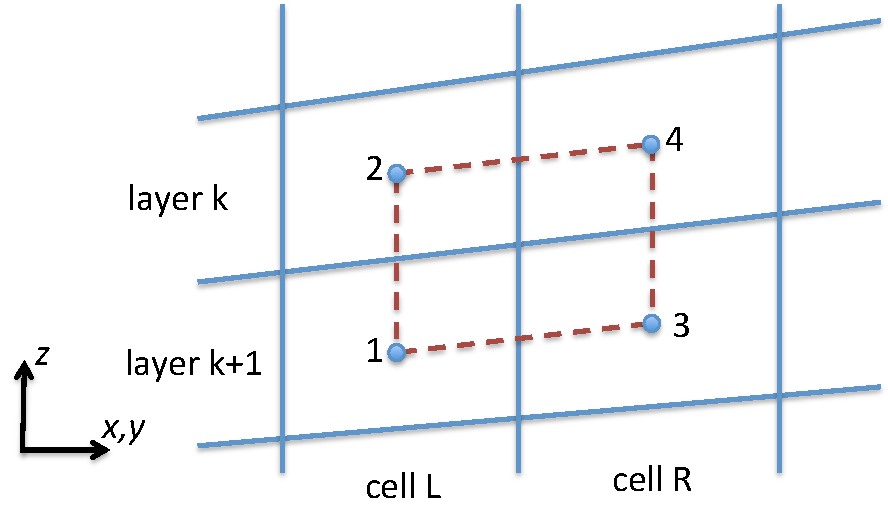
\includegraphics[width=3.5in]{ocean/figures/common_level.pdf}
\caption{Vertical cross-section of ocean grid cells, showing index locations for common level method.  The dots are placed at cell centers in the horizontal and layer mid-depth in the vertical.}
\label{oceanFigure:common level}
\end{figure}

{\bf \large config\_pressure\_gradient\_type = 'Jacobian\_from\_density'}\\
In this formulation the pressure gradient is rewritten in terms of a sea surface height gradient and the vertical integral of a Jacobian,
\begin{eqnarray}
\label{ocean:grad p Jacobian}
- \frac{1}{\rho_0}\nabla_z p &=& - \frac{\rho_s g}{\rho_0}\nabla_s \zeta - \frac{g}{\rho_0}\int_z^\zeta {\mathcal J}(\rho,z)ds, \\
{\mathcal J}(\rho,z) &=& \left. \frac{\partial \rho}{\partial x} \right|_s \frac{\partial z}{\partial s} 
 - \frac{\partial \rho}{\partial s}  \left. \frac{\partial z}{\partial x} \right|_s 
\end{eqnarray}
where $x$ is a general horizontal direction between two cell centers and $s$ is the vertical coordinate reference, i.e.\ $s$ is constant within a layer.  There are many methods to discretize the Jacobian term.  In the common level method, the density is linearly interpolated or extrapolated within each vertical column to a common level $z_\gamma$ (see Figure \ref{oceanFigure:common level}):
\begin{eqnarray}
- \int_z^\zeta {\mathcal J}(\rho,z)ds &=& \overline{\Delta z} \left( \rho^L - \rho^R \right) \\
\overline{\Delta z} &=& \frac{1}{2} \left(z_2-z_1 + z_4-z_3\right) \\
\rho^L &=& \frac{\rho_1\left(z_2-z_\gamma\right) + \rho_2\left(z_\gamma-z_1\right) }{z_2-z_1}\\
\rho^R &=& \frac{\rho_3\left(z_4-z_\gamma\right) + \rho_4\left(z_\gamma-z_3\right) }{z_4-z_3}\\
z_\gamma &=& \left(1-\gamma\right)z_* + \gamma z_c \\
z_* &=&  \frac{z_4 z_2-z_3z_1}{z_4-z_3 + z_2-z_1} \\
z_c &=&  \frac{z_1+z_2+z_3+z_4}{4} 
\end{eqnarray}
where $z_c$ is the depth for the weighted Jacobian method by \citet{Song98mwr}, and $z_*$ is the depth for the standard Jacobian method, which is the depth of intersection of the diagonals of the trapezoidal element in Figure \ref{oceanFigure:common level}.  Here $\gamma$ weights the choice between these two methods for computing the common level $z_\gamma$.  This formulation for the pressure gradient is described in detail in \citet{Shchepetkin_McWilliams03jgr}, Section 2, method 2, and Section 4.  They found that a coefficient of $\gamma=0.5$, which gives equal weights to the standard and weighted Jacobian methods, minimizes the errors in a seamount test problem.

{\bf \large config\_pressure\_gradient\_type = 'Jacobian\_from\_TS'}\\
This formulation is the same as the previous, except that the Jacobian is computed using a linear expansion in potential temperature and salinity.  This option must be used when layers are extremely tilted, such as with sigma coordinates or under an ice shelf, in combination with a nonlinear equation of state.
\begin{eqnarray}
 {\mathcal J}(\rho,z) &=& -\alpha  {\mathcal J}(\theta,z) + \beta  {\mathcal J}(S,z), 
\end{eqnarray}
where
\begin{eqnarray}
\alpha\left( \theta, S, p\right) &=&  -\left. \frac{\partial \rho}{\partial \theta} \right|_{S,p} \\
\beta\left( \theta, S, p\right) &=&  \left. \frac{\partial \rho}{\partial S} \right|_{\theta,p} 
\end{eqnarray}
are the thermal expansion and saline contraction coefficients, computed at a particular  $\left(\theta, S, p\right)$ by the equation of state \citep[eqn 7.16]{Shchepetkin_McWilliams03jgr}.

{\bf \large config\_pressure\_gradient\_type = 'MontgomeryPotential'}\\
For isopycnal vertical coordinates, the user may choose to use the Montgomery potential,
\begin{equation}
\label{ocean:Montgomery Potential}
M = \frac{1}{\rho}p+gz
\end{equation}
and replace the pressure terms above with
\begin{equation}
- \nabla_s M.
\end{equation}
See \citet[section 2.1]{Higdon05jcp} for details on the derivation and computation of the Montgomery potential.

% {\bf \large config\_pressure\_gradient\_type = 'MontgomeryPotential\_and\_density'}
% Same as previous, but this formulation includes an extra term,
% \begin{equation}
% - \nabla_s M + p \nabla_s\left(\frac{1}{\rho} \right),
% \end{equation}
% as described by \citet{Bleck02om}, eqn 1 and end of Appendix A.  This formulation has not been extensively tested and is not supported at this time.

\vspace{0.5in}
{\small
\begin{center}
\begin{longtable}{| p{2.0in} || p{4.0in} |}
	\hline
	{\bf Name} & {\bf Description} \endfirsthead
	\hline 
	{\bf Name} & {\bf Description} (Continued) \endhead
	\hline
	\hline
	\hyperref[sec:nm_sec_config_pressure_gradient_type]{config\_pressure\_gradient\_type} & Form of pressure gradient terms in momentum equation. For most applications, the gradient of pressure and layer mid-depth are appropriate.  For isopycnal coordinates, one may use the gradient of the Montgomery potential. \\
	\hline
	\hyperref[sec:nm_sec_config_density0]{config\_density0} &  Density used as a coefficient of the pressure gradient terms,  $\rho_0$ . This is a constant due to the Boussinesq approximation. \\
	\hline
	\hyperref[sec:nm_sec_config_common_level_weight]{config\_common\_level\_weight} &  The weight between standard Jacobian and weighted Jacobian,  $\gamma$ . \\
	\hline
\end{longtable}
\end{center}
}
\subsection[eos]{eos}
\label{subsec:forward_nm_tab_eos}
Two forms of EOS are supported. The full EOS from \cite{Jackett_McDougall95jaot} and a linear EOS.

\vspace{0.5in}
{\small
\begin{center}
\begin{longtable}{| p{2.0in} || p{4.0in} |}
	\hline
	{\bf Name} & {\bf Description} \endfirsthead
	\hline 
	{\bf Name} & {\bf Description} (Continued) \endhead
	\hline
	\hline
	\hyperref[sec:nm_sec_config_eos_type]{config\_eos\_type} & Character string to choose EOS formulation \\
	\hline
\end{longtable}
\end{center}
}
\subsection[eos\_linear]{eos\_linear}
\label{subsec:forward_nm_tab_eos_linear}
The linear equation of state (leos) is specified as follows:
\begin{equation}
\rho = \rho_{ref} - \alpha_{leos}(T-T_{ref})+\beta_{leos}(S-S_{ref})
\end{equation}
\vspace{0.5in}
{\small
\begin{center}
\begin{longtable}{| p{2.0in} || p{4.0in} |}
	\hline
	{\bf Name} & {\bf Description} \endfirsthead
	\hline 
	{\bf Name} & {\bf Description} (Continued) \endhead
	\hline
	\hline
	\hyperref[sec:nm_sec_config_eos_linear_alpha]{config\_eos\_linear\_alpha} & Linear thermal expansion coefficient \\
	\hline
	\hyperref[sec:nm_sec_config_eos_linear_beta]{config\_eos\_linear\_beta} & Linear haline contraction coefficient \\
	\hline
	\hyperref[sec:nm_sec_config_eos_linear_Tref]{config\_eos\_linear\_Tref} & Reference temperature \\
	\hline
	\hyperref[sec:nm_sec_config_eos_linear_Sref]{config\_eos\_linear\_Sref} & Reference salinity \\
	\hline
	\hyperref[sec:nm_sec_config_eos_linear_densityref]{config\_eos\_linear\_densityref} & Reference density, i.e. density when T=Tref and S=Sref \\
	\hline
\end{longtable}
\end{center}
}
\subsection[split\_explicit\_ts]{split\_explicit\_ts}
\label{subsec:forward_nm_tab_split_explicit_ts}
The split explicit time-stepping method solves the barotropic (vertically-integrated) velocities separately from the remaining baroclinic velocities.  The time step for the barotropic solve is limited by fast surface gravity waves, and so is subcycled within a large timestep of the baroclinic velocity solve.  This provides a 10 to 12-times speed-up over fourth-order Runge-Kutta time stepping.

A single large timestep in the split explicit algorithm may be summarized as
\begin{itemize}
\item Stage 1: solve for baroclinic velocity (3D)
\item Stage 2: solve for barotropic velocity (2D) with explicit sub-cycling
\item Stage 3: update thickness, tracers, density and pressure
\end{itemize}
The algorithm includes iterations within stage 1, within each subcycle of stage 2, and over the full three-stage process.  Further details are provided in \citet[Appendix A.5]{Ringler_ea13om}

\vspace{0.5in}
{\small
\begin{center}
\begin{longtable}{| p{2.0in} || p{4.0in} |}
	\hline
	{\bf Name} & {\bf Description} \endfirsthead
	\hline 
	{\bf Name} & {\bf Description} (Continued) \endhead
	\hline
	\hline
	\hyperref[sec:nm_sec_config_n_ts_iter]{config\_n\_ts\_iter} & number of large iterations over stages 1-3 \\
	\hline
	\hyperref[sec:nm_sec_config_n_bcl_iter_beg]{config\_n\_bcl\_iter\_beg} & number of iterations of stage 1 (baroclinic solve) on the first split-explicit iteration \\
	\hline
	\hyperref[sec:nm_sec_config_n_bcl_iter_mid]{config\_n\_bcl\_iter\_mid} & number of iterations of stage 1 (baroclinic solve) on any split-explicit iterations between first and last \\
	\hline
	\hyperref[sec:nm_sec_config_n_bcl_iter_end]{config\_n\_bcl\_iter\_end} & number of iterations of stage 1 (baroclinic solve) on the last split-explicit iteration \\
	\hline
	\hyperref[sec:nm_sec_config_n_btr_subcycles]{config\_n\_btr\_subcycles} & number of barotropic subcycles in stage 2 \\
	\hline
	\hyperref[sec:nm_sec_config_n_btr_cor_iter]{config\_n\_btr\_cor\_iter} & number of iterations of the velocity corrector step in stage 2 \\
	\hline
	\hyperref[sec:nm_sec_config_vel_correction]{config\_vel\_correction} & If true, the velocity correction term is included in the horizontal advection of thickness and tracers \\
	\hline
	\hyperref[sec:nm_sec_config_btr_subcycle_loop_factor]{config\_btr\_subcycle\_loop\_facto-}\hyperref[sec:nm_sec_config_btr_subcycle_loop_factor]{r}&  Barotropic subcycles proceed from  $t$  to  $t+n\Delta t$ , where  $n$  is this configuration option. \\
	\hline
	\hyperref[sec:nm_sec_config_btr_gam1_velWt1]{config\_btr\_gam1\_velWt1} & Weighting of velocity in the SSH predictor step in stage 2. When zero, previous subcycle time is used; when one, new subcycle time is used. \\
	\hline
	\hyperref[sec:nm_sec_config_btr_gam2_SSHWt1]{config\_btr\_gam2\_SSHWt1} & Weighting of SSH in the velocity corrector step in stage 2. When zero, previous subcycle time is used; when one, new subcycle time is used. \\
	\hline
	\hyperref[sec:nm_sec_config_btr_gam3_velWt2]{config\_btr\_gam3\_velWt2} & Weighting of velocity in the SSH corrector step in stage 2. When zero, previous subcycle time is used; when one, new subcycle time is used. \\
	\hline
	\hyperref[sec:nm_sec_config_btr_solve_SSH2]{config\_btr\_solve\_SSH2} & If true, execute the SSH corrector step in stage 2 \\
	\hline
\end{longtable}
\end{center}
}
\subsection[testing]{testing}
\label{subsec:forward_nm_tab_testing}
\section{Testing}
\label{sec:testing}

\vspace{0.5in}
{\small
\begin{center}
\begin{longtable}{| p{2.0in} || p{4.0in} |}
	\hline
	{\bf Name} & {\bf Description} \endfirsthead
	\hline 
	{\bf Name} & {\bf Description} (Continued) \endhead
	\hline
	\hline
	\hyperref[sec:nm_sec_config_conduct_tests]{config\_conduct\_tests} & If true, run testing suite. This is the overarching control on the test suite. Individual flags must be set to true below to conduct each test. \\
	\hline
	\hyperref[sec:nm_sec_config_test_tensors]{config\_test\_tensors} & If true, tensor operations are tested upon start-up. \\
	\hline
	\hyperref[sec:nm_sec_config_tensor_test_function]{config\_tensor\_test\_function} & Character string to choose tensor test fuction \\
	\hline
\end{longtable}
\end{center}
}
\subsection[debug]{debug}
\label{subsec:forward_nm_tab_debug}
At run-time a user can enable debugging features within MPAS-Ocean. These
features include disabling any tendencies to help determine why an issue might
be happening. Debugging options also include various checks on certain fields,
and the ability to prescribe both a thickness and velocity field at run-time
which are constant throughout a simulation. All options that control these
debugging features are specified within the debug namelist record.

\vspace{0.5in}
{\small
\begin{center}
\begin{longtable}{| p{2.0in} || p{4.0in} |}
	\hline
	{\bf Name} & {\bf Description} \endfirsthead
	\hline 
	{\bf Name} & {\bf Description} (Continued) \endhead
	\hline
	\hline
	\hyperref[sec:nm_sec_config_disable_redi_k33]{config\_disable\_redi\_k33} & If true, disables k33 portion of Redi neutral surface mixing. \\
	\hline
	\hyperref[sec:nm_sec_config_disable_redi_horizontal_term1]{config\_disable\_redi\_horizontal\_t-}\hyperref[sec:nm_sec_config_disable_redi_horizontal_term1]{erm1}& If true, disables first term in horizonal mixing of Redi neutral surface mixing. \\
	\hline
	\hyperref[sec:nm_sec_config_disable_redi_horizontal_term2]{config\_disable\_redi\_horizontal\_t-}\hyperref[sec:nm_sec_config_disable_redi_horizontal_term2]{erm2}& If true, disables first term in horizonal mixing of Redi neutral surface mixing. \\
	\hline
	\hyperref[sec:nm_sec_config_disable_redi_horizontal_term3]{config\_disable\_redi\_horizontal\_t-}\hyperref[sec:nm_sec_config_disable_redi_horizontal_term3]{erm3}& If true, disables first term in horizonal mixing of Redi neutral surface mixing. \\
	\hline
	\hyperref[sec:nm_sec_config_check_zlevel_consistency]{config\_check\_zlevel\_consistency} & Enables a run-time check for consistency for a zlevel grid. Ensures relevant variables correctly define the bottom of the ocean. \\
	\hline
	\hyperref[sec:nm_sec_config_filter_btr_mode]{config\_filter\_btr\_mode} & Enables filtering of the barotropic mode. \\
	\hline
	\hyperref[sec:nm_sec_config_prescribe_velocity]{config\_prescribe\_velocity} & Enables a prescribed velocity field. This velocity field is read on input, and remains constant through a simulation. \\
	\hline
	\hyperref[sec:nm_sec_config_prescribe_thickness]{config\_prescribe\_thickness} & Enables a prescribed thickness field. This thickness field is read on input, and remains constant through a simulation. \\
	\hline
	\hyperref[sec:nm_sec_config_include_KE_vertex]{config\_include\_KE\_vertex} & If true, the kinetic energy in each cell is computed by blending cell-based and vertex-based values of kinetic energy. \\
	\hline
	\hyperref[sec:nm_sec_config_check_tracer_monotonicity]{config\_check\_tracer\_monotonici-}\hyperref[sec:nm_sec_config_check_tracer_monotonicity]{ty}& Enables a change on tracer monotonicity at the end of the monotonic advection routine. Only used if config\_monotonic is set to .true. \\
	\hline
	\hyperref[sec:nm_sec_config_disable_thick_all_tend]{config\_disable\_thick\_all\_tend} & Disables all tendencies on the thickness field. \\
	\hline
	\hyperref[sec:nm_sec_config_disable_thick_hadv]{config\_disable\_thick\_hadv} & Disable tendencies on the thickness field from horizontal advection. \\
	\hline
	\hyperref[sec:nm_sec_config_disable_thick_vadv]{config\_disable\_thick\_vadv} & Disables tendencies on the thickness field from vertical advection. \\
	\hline
	\hyperref[sec:nm_sec_config_disable_thick_sflux]{config\_disable\_thick\_sflux} & Disables tendencies on the thickness field from surface fluxes. \\
	\hline
	\hyperref[sec:nm_sec_config_disable_vel_all_tend]{config\_disable\_vel\_all\_tend} & Disables all tendencies on the velocity field. \\
	\hline
	\hyperref[sec:nm_sec_config_disable_vel_coriolis]{config\_disable\_vel\_coriolis} & Diables tendencies on the velocity field from the Coriolis force. \\
	\hline
	\hyperref[sec:nm_sec_config_disable_vel_pgrad]{config\_disable\_vel\_pgrad} & Disables tendencies on the velocity field from the horizontal pressure gradient. \\
	\hline
	\hyperref[sec:nm_sec_config_disable_vel_hmix]{config\_disable\_vel\_hmix} & Disables tendencies on the velocity field from horizontal mixing. \\
	\hline
	\hyperref[sec:nm_sec_config_disable_vel_windstress]{config\_disable\_vel\_windstress} & Disables tendencies on the velocity field from horizontal wind stress. \\
	\hline
	\hyperref[sec:nm_sec_config_disable_vel_vmix]{config\_disable\_vel\_vmix} & Disables tendencies on the velocity field from vertical mixing. \\
	\hline
	\hyperref[sec:nm_sec_config_disable_vel_vadv]{config\_disable\_vel\_vadv} & Disables tendencies on the velocity field from vertical advection. \\
	\hline
	\hyperref[sec:nm_sec_config_disable_tr_all_tend]{config\_disable\_tr\_all\_tend} & Disables all tendencies on tracer fields. \\
	\hline
	\hyperref[sec:nm_sec_config_disable_tr_adv]{config\_disable\_tr\_adv} & Disables tendencies on tracer fields from advection, both horizontal and vertical. \\
	\hline
	\hyperref[sec:nm_sec_config_disable_tr_hmix]{config\_disable\_tr\_hmix} & Disables tendencies on tracer fields from horizontal mixing. \\
	\hline
	\hyperref[sec:nm_sec_config_disable_tr_vmix]{config\_disable\_tr\_vmix} & Disables tendencies on tracer fields from vertical mixing. \\
	\hline
	\hyperref[sec:nm_sec_config_disable_tr_sflux]{config\_disable\_tr\_sflux} & Disables tendencies on tracer fields from surface fluxes. \\
	\hline
	\hyperref[sec:nm_sec_config_disable_tr_nonlocalflux]{config\_disable\_tr\_nonlocalflux} & Disables tendencies on the tracer fields from CVMix/KPP nonlocal fluxes. \\
	\hline
\end{longtable}
\end{center}
}
\subsection[global\_stats]{global\_stats}
\label{subsec:forward_nm_tab_global_stats}
The global statistics analysis member computes the same statistics as those listed in section \ref{sec:global_statistics}.  The global statistics output is written to a netcdf file, as specified in the streams.ocean\_forward file for forward mode, and the streams.ocean\_analysis file for analysis mode.

\vspace{0.5in}
{\small
\begin{center}
\begin{longtable}{| p{2.0in} || p{4.0in} |}
	\hline
	{\bf Name} & {\bf Description} \endfirsthead
	\hline 
	{\bf Name} & {\bf Description} (Continued) \endhead
	\hline
	\hline
	\hyperref[sec:nm_sec_config_use_global_stats]{config\_use\_global\_stats} & If true, ocean analysis member global\_stats is called. \\
	\hline
	\hyperref[sec:nm_sec_config_global_stats_compute_interval]{config\_global\_stats\_compute\_int-}\hyperref[sec:nm_sec_config_global_stats_compute_interval]{erval}& Timestamp determining how often analysis member computation should be performed. \\
	\hline
	\hyperref[sec:nm_sec_config_global_stats_compute_startup]{config\_global\_stats\_compute\_st-}\hyperref[sec:nm_sec_config_global_stats_compute_startup]{artup}& Logical flag determining if an analysis member computation occurs on start-up. \\
	\hline
\end{longtable}
\end{center}
}
\subsection[zonal\_mean]{zonal\_mean}
\label{subsec:forward_nm_tab_zonal_mean}
The zonal mean analysis member computes the zonal means of several variables.  The width and number of latitude bins are specified by the flags below.  The zonal mean output is written to a netcdf file, as specified in streams.ocean\_forward file for forward mode, and the streams.ocean\_analysis file for analysis mode.

\vspace{0.5in}
{\small
\begin{center}
\begin{longtable}{| p{2.0in} || p{4.0in} |}
	\hline
	{\bf Name} & {\bf Description} \endfirsthead
	\hline 
	{\bf Name} & {\bf Description} (Continued) \endhead
	\hline
	\hline
	\hyperref[sec:nm_sec_config_use_zonal_mean]{config\_use\_zonal\_mean} & If true, ocean analysis member zonal\_mean is called. \\
	\hline
	\hyperref[sec:nm_sec_config_zonal_mean_compute_interval]{config\_zonal\_mean\_compute\_inte-}\hyperref[sec:nm_sec_config_zonal_mean_compute_interval]{rval}& Timestamp determining how often analysis member computation should be performed. \\
	\hline
	\hyperref[sec:nm_sec_config_zonal_mean_compute_startup]{config\_zonal\_mean\_compute\_sta-}\hyperref[sec:nm_sec_config_zonal_mean_compute_startup]{rtup}& Logical flag determining if an analysis member computation occurs on start-up. \\
	\hline
	\hyperref[sec:nm_sec_config_number_zonal_mean_bins]{config\_number\_zonal\_mean\_bins} & Number of bins used for zonal mean.  Must be less than or equal to the dimension nZonalMeanBins (set in Registry). \\
	\hline
	\hyperref[sec:nm_sec_config_min_zonal_mean_bin]{config\_min\_zonal\_mean\_bin} & minimum bin boundary value.  If set to -1.0e34, the minimum value in the domain is found. \\
	\hline
	\hyperref[sec:nm_sec_config_max_zonal_mean_bin]{config\_max\_zonal\_mean\_bin} & maximum bin boundary value.  If set to -1.0e34, the maximum value in the domain is found. \\
	\hline
\end{longtable}
\end{center}
}
\section[Variable definitions]{\hyperref[chap:variable_sections]{Variable definitions}}
\label{sec:forward_variable_tables}
Embedded links point to more detailed variable information in the appendix.
\subsection[state]{\hyperref[sec:var_sec_state]{state}}
\label{subsec:forward_var_tab_state}
The state data structure contains a set of prognostic and diagnostic fields
that are time dependent. The fields contained inside of state have two time
levels available in the default version of MPAS-Ocean.

\vspace{0.5in}
{\small
\begin{center}
\begin{longtable}{| p{2.0in} | p{4.0in} |}
	\hline
	{\bf Name} & {\bf Description} \endfirsthead
	\hline 
	{\bf Name} & {\bf Description} (Continued) \endhead
	\hline
	\hyperref[subsec:var_sec_state_temperature]{temperature} & potential temperature \\
	\hline
	\hyperref[subsec:var_sec_state_salinity]{salinity} & salinity \\
	\hline
	\hyperref[subsec:var_sec_state_tracer1]{tracer1} & tracer \\
	\hline
	\hyperref[subsec:var_sec_state_normalVelocity]{normalVelocity} & horizonal velocity, normal component to an edge \\
	\hline
	\hyperref[subsec:var_sec_state_layerThickness]{layerThickness} & layer thickness \\
	\hline
	\hyperref[subsec:var_sec_state_ssh]{ssh} & sea surface height \\
	\hline
	\hyperref[subsec:var_sec_state_highFreqThickness]{highFreqThickness} & high frequency-filtered layer thickness \\
	\hline
	\hyperref[subsec:var_sec_state_lowFreqDivergence]{lowFreqDivergence} & low frequency-filtered divergence \\
	\hline
	\hyperref[subsec:var_sec_state_normalBarotropicVelocity]{normalBarotropicVelocity} & barotropic velocity, used in split-explicit time-stepping \\
	\hline
	\hyperref[subsec:var_sec_state_normalBarotropicVelocitySubcycle]{normalBarotropicVelocitySubcy-}\hyperref[subsec:var_sec_state_normalBarotropicVelocitySubcycle]{cle  }& barotropic velocity, used in subcycling in stage 2 of split-explicit time-stepping \\
	\hline
	\hyperref[subsec:var_sec_state_sshSubcycle]{sshSubcycle} & sea surface height, used in subcycling in stage 2 of split-explicit time-stepping \\
	\hline
	\hyperref[subsec:var_sec_state_normalBaroclinicVelocity]{normalBaroclinicVelocity} & baroclinic velocity, used in split-explicit time-stepping \\
	\hline
\end{longtable}
\end{center}
}
\subsection[mesh]{\hyperref[sec:var_sec_mesh]{mesh}}
\label{subsec:forward_var_tab_mesh}
The mesh data type contains a single time level. The fields inside the mesh
structure are not assumed to be time dependent. This data structure contains
fields that describe the mesh, and the connectivity of the mesh. Several of the
fields contained in this structure are shared throughout all MPAS dynamical
cores.

\vspace{0.5in}
{\small
\begin{center}
\begin{longtable}{| p{2.0in} | p{4.0in} |}
	\hline
	{\bf Name} & {\bf Description} \endfirsthead
	\hline 
	{\bf Name} & {\bf Description} (Continued) \endhead
	\hline
	\hyperref[subsec:var_sec_mesh_latCell]{latCell} & Latitude location of cell centers in radians. \\
	\hline
	\hyperref[subsec:var_sec_mesh_lonCell]{lonCell} & Longitude location of cell centers in radians. \\
	\hline
	\hyperref[subsec:var_sec_mesh_xCell]{xCell} & X Coordinate in cartesian space of cell centers. \\
	\hline
	\hyperref[subsec:var_sec_mesh_yCell]{yCell} & Y Coordinate in cartesian space of cell centers. \\
	\hline
	\hyperref[subsec:var_sec_mesh_zCell]{zCell} & Z Coordinate in cartesian space of cell centers. \\
	\hline
	\hyperref[subsec:var_sec_mesh_indexToCellID]{indexToCellID} & List of global cell IDs. \\
	\hline
	\hyperref[subsec:var_sec_mesh_latEdge]{latEdge} & Latitude location of edge midpoints in radians. \\
	\hline
	\hyperref[subsec:var_sec_mesh_lonEdge]{lonEdge} & Longitude location of edge midpoints in radians. \\
	\hline
	\hyperref[subsec:var_sec_mesh_xEdge]{xEdge} & X Coordinate in cartesian space of edge midpoints. \\
	\hline
	\hyperref[subsec:var_sec_mesh_yEdge]{yEdge} & Y Coordinate in cartesian space of edge midpoints. \\
	\hline
	\hyperref[subsec:var_sec_mesh_zEdge]{zEdge} & Z Coordinate in cartesian space of edge midpoints. \\
	\hline
	\hyperref[subsec:var_sec_mesh_indexToEdgeID]{indexToEdgeID} & List of global edge IDs. \\
	\hline
	\hyperref[subsec:var_sec_mesh_latVertex]{latVertex} & Latitude location of vertices in radians. \\
	\hline
	\hyperref[subsec:var_sec_mesh_lonVertex]{lonVertex} & Longitude location of vertices in radians. \\
	\hline
	\hyperref[subsec:var_sec_mesh_xVertex]{xVertex} & X Coordinate in cartesian space of vertices. \\
	\hline
	\hyperref[subsec:var_sec_mesh_yVertex]{yVertex} & Y Coordinate in cartesian space of vertices. \\
	\hline
	\hyperref[subsec:var_sec_mesh_zVertex]{zVertex} & Z Coordinate in cartesian space of vertices. \\
	\hline
	\hyperref[subsec:var_sec_mesh_indexToVertexID]{indexToVertexID} & List of global vertex IDs. \\
	\hline
	\hyperref[subsec:var_sec_mesh_meshDensity]{meshDensity} & Value of density function used to generate a particular mesh at cell centers. \\
	\hline
	\hyperref[subsec:var_sec_mesh_meshScalingDel2]{meshScalingDel2} & Coefficient to Laplacian mixing terms in momentum and tracer equations, so that viscosity and diffusion scale with mesh. \\
	\hline
	\hyperref[subsec:var_sec_mesh_meshScalingDel4]{meshScalingDel4} & Coefficient to biharmonic mixing terms in momentum and tracer equations, so that biharmonic viscosity and diffusion coefficients scale with mesh. \\
	\hline
	\hyperref[subsec:var_sec_mesh_meshScaling]{meshScaling} & Coefficient used for mesh scaling, such as the Leith parameter. \\
	\hline
	\hyperref[subsec:var_sec_mesh_cellsOnEdge]{cellsOnEdge} & List of cells that straddle each edge. \\
	\hline
	\hyperref[subsec:var_sec_mesh_nEdgesOnCell]{nEdgesOnCell} & Number of edges that border each cell. \\
	\hline
	\hyperref[subsec:var_sec_mesh_nEdgesOnEdge]{nEdgesOnEdge} & Number of edges that surround each of the cells that straddle each edge. These edges are used to reconstruct the tangential velocities. \\
	\hline
	\hyperref[subsec:var_sec_mesh_edgesOnCell]{edgesOnCell} & List of edges that border each cell. \\
	\hline
	\hyperref[subsec:var_sec_mesh_edgesOnEdge]{edgesOnEdge} & List of edges that border each of the cells that straddle each edge. \\
	\hline
	\hyperref[subsec:var_sec_mesh_weightsOnEdge]{weightsOnEdge} & Reconstruction weights associated with each of the edgesOnEdge. \\
	\hline
	\hyperref[subsec:var_sec_mesh_dvEdge]{dvEdge} & Length of each edge, computed as the distance between verticesOnEdge. \\
	\hline
	\hyperref[subsec:var_sec_mesh_dcEdge]{dcEdge} & Length of each edge, computed as the distance between cellsOnEdge. \\
	\hline
	\hyperref[subsec:var_sec_mesh_angleEdge]{angleEdge} & Angle the edge normal makes with local eastward direction. \\
	\hline
	\hyperref[subsec:var_sec_mesh_areaCell]{areaCell} & Area of each cell in the primary grid. \\
	\hline
	\hyperref[subsec:var_sec_mesh_areaTriangle]{areaTriangle} & Area of each cell (triangle) in the dual grid. \\
	\hline
	\hyperref[subsec:var_sec_mesh_edgeNormalVectors]{edgeNormalVectors} & Normal unit vector defined at an edge. \\
	\hline
	\hyperref[subsec:var_sec_mesh_edgeTangentVectors]{edgeTangentVectors} & Tangent unit vector defined at an edge. \\
	\hline
	\hyperref[subsec:var_sec_mesh_localVerticalUnitVectors]{localVerticalUnitVectors} & Unit surface normal vectors defined at cell centers. \\
	\hline
	\hyperref[subsec:var_sec_mesh_cellTangentPlane]{cellTangentPlane} & The two vectors that define a tangent plane at a cell center. \\
	\hline
	\hyperref[subsec:var_sec_mesh_cellsOnCell]{cellsOnCell} & List of cells that neighbor each cell. \\
	\hline
	\hyperref[subsec:var_sec_mesh_verticesOnCell]{verticesOnCell} & List of vertices that border each cell. \\
	\hline
	\hyperref[subsec:var_sec_mesh_verticesOnEdge]{verticesOnEdge} & List of vertices that straddle each edge. \\
	\hline
	\hyperref[subsec:var_sec_mesh_edgesOnVertex]{edgesOnVertex} & List of edges that share a vertex as an endpoint. \\
	\hline
	\hyperref[subsec:var_sec_mesh_cellsOnVertex]{cellsOnVertex} & List of cells that share a vertex. \\
	\hline
	\hyperref[subsec:var_sec_mesh_kiteAreasOnVertex]{kiteAreasOnVertex} & Area of the portions of each dual cell that are part of each cellsOnVertex. \\
	\hline
	\hyperref[subsec:var_sec_mesh_fEdge]{fEdge} & Coriolis parameter at edges. \\
	\hline
	\hyperref[subsec:var_sec_mesh_fVertex]{fVertex} & Coriolis parameter at vertices. \\
	\hline
	\hyperref[subsec:var_sec_mesh_fCell]{fCell} & Coriolis parameter at cell centers. \\
	\hline
	\hyperref[subsec:var_sec_mesh_bottomDepth]{bottomDepth} & Depth of the bottom of the ocean. Given as a positive distance from sea level. \\
	\hline
	\hyperref[subsec:var_sec_mesh_derivTwo]{derivTwo} & Value of the second derivative of the polynomial used for reconstruction of cell center quantities at edges. \\
	\hline
	\hyperref[subsec:var_sec_mesh_advCoefs]{advCoefs} & Weighting coefficients used for reconstruction of cell center quantities at edges. Used in advection routines. \\
	\hline
	\hyperref[subsec:var_sec_mesh_advCoefs3rd]{advCoefs3rd} & Wegihting coefficients used for reconstruction of cell center quantities at edges. Used in advection routines. \\
	\hline
	\hyperref[subsec:var_sec_mesh_advCellsForEdge]{advCellsForEdge} & List of cells used to reconstruct a cell quantity at an edge. Used in advection routines. \\
	\hline
	\hyperref[subsec:var_sec_mesh_nAdvCellsForEdge]{nAdvCellsForEdge} & Number of cells used in reconstruction of cell center quantities at an edge. Used in advection routines. \\
	\hline
	\hyperref[subsec:var_sec_mesh_highOrderAdvectionMask]{highOrderAdvectionMask} & Mask for high order advection. Values are 1 if high order is used, and 0 if not. \\
	\hline
	\hyperref[subsec:var_sec_mesh_coeffs_reconstruct]{coeffs\_reconstruct} & Coefficients to reconstruct velocity vectors at cells centers. \\
	\hline
	\hyperref[subsec:var_sec_mesh_maxLevelCell]{maxLevelCell} & Index to the last active ocean cell in each column. \\
	\hline
	\hyperref[subsec:var_sec_mesh_maxLevelEdgeTop]{maxLevelEdgeTop} & Index to the last edge in a column with active ocean cells on both sides of it. \\
	\hline
	\hyperref[subsec:var_sec_mesh_maxLevelEdgeBot]{maxLevelEdgeBot} & Index to the last edge in a column with at least one active ocean cell on either side of it. \\
	\hline
	\hyperref[subsec:var_sec_mesh_maxLevelVertexTop]{maxLevelVertexTop} & Index to the last vertex in a column with all active cells around it. \\
	\hline
	\hyperref[subsec:var_sec_mesh_maxLevelVertexBot]{maxLevelVertexBot} & Index to the last vertex in a column with at least one active ocean cell around it. \\
	\hline
	\hyperref[subsec:var_sec_mesh_refBottomDepth]{refBottomDepth} & Reference depth of ocean for each vertical level. Used in 'z-level' type runs. \\
	\hline
	\hyperref[subsec:var_sec_mesh_refBottomDepthTopOfCell]{refBottomDepthTopOfCell} & Reference depth of ocean for each vertical interface. Used in 'z-level' type runs. \\
	\hline
	\hyperref[subsec:var_sec_mesh_vertCoordMovementWeights]{vertCoordMovementWeights} & Weights used for distribution of sea surface heigh purturbations through multiple vertical levels. \\
	\hline
	\hyperref[subsec:var_sec_mesh_boundaryEdge]{boundaryEdge} & Mask for determining boundary edges. A boundary edge has only one active ocean cell neighboring it. \\
	\hline
	\hyperref[subsec:var_sec_mesh_boundaryVertex]{boundaryVertex} & Mask for determining boundary vertices. A boundary vertex has at least one inactive cell neighboring it. \\
	\hline
	\hyperref[subsec:var_sec_mesh_boundaryCell]{boundaryCell} & Mask for determining boundary cells. A boundary cell has at least one inactive cell neighboring it. \\
	\hline
	\hyperref[subsec:var_sec_mesh_edgeMask]{edgeMask} & Mask on edges that determines if computations should be done on edge. \\
	\hline
	\hyperref[subsec:var_sec_mesh_vertexMask]{vertexMask} & Mask on vertices that determines if computations should be done on vertice. \\
	\hline
	\hyperref[subsec:var_sec_mesh_cellMask]{cellMask} & Mask on cells that determines if computations should be done on cell. \\
	\hline
	\hyperref[subsec:var_sec_mesh_temperatureRestore]{temperatureRestore} & Temperature restoring field, for restoring temperature at the surface. \\
	\hline
	\hyperref[subsec:var_sec_mesh_salinityRestore]{salinityRestore} & Salinity restoring field, for restoring salinity at the surface. \\
	\hline
	\hyperref[subsec:var_sec_mesh_edgeSignOnCell]{edgeSignOnCell} & Sign of edge contributions to a cell for each edge on cell. Used for bit-reproducible loops. Represents directionality of vector connecting cells. \\
	\hline
	\hyperref[subsec:var_sec_mesh_edgeSignOnVertex]{edgeSignOnVertex} & Sign of edge contributions to a vertex for each edge on vertex. Used for bit-reproducible loops. Represents directionality of vector connecting vertices. \\
	\hline
	\hyperref[subsec:var_sec_mesh_kiteIndexOnCell]{kiteIndexOnCell} & Index of kite in dual grid, based on verticesOnCell. \\
	\hline
\end{longtable}
\end{center}
}
\subsection[verticalMesh]{\hyperref[sec:var_sec_verticalMesh]{verticalMesh}}
\label{subsec:forward_var_tab_verticalMesh}
The vertical mesh data type contains a single time level. The fields inside the
vertical mesh structure are not assumed to be time dependent. This data
structure contains fields that describe the vertical mesh and are used for
various types of vertical meshes.

\vspace{0.5in}
{\small
\begin{center}
\begin{longtable}{| p{2.0in} | p{4.0in} |}
	\hline
	{\bf Name} & {\bf Description} \endfirsthead
	\hline 
	{\bf Name} & {\bf Description} (Continued) \endhead
	\hline
	\hyperref[subsec:var_sec_verticalMesh_restingThickness]{restingThickness} & Layer thickness when the ocean is at rest, i.e. without SSH or internal perturbations. \\
	\hline
	\hyperref[subsec:var_sec_verticalMesh_refZMid]{refZMid} & Reference mid z-coordinate of ocean for each vertical level. This has a negative value. \\
	\hline
	\hyperref[subsec:var_sec_verticalMesh_refLayerThickness]{refLayerThickness} & Reference layerThickness of ocean for each vertical level. \\
	\hline
\end{longtable}
\end{center}
}
\subsection[tend]{\hyperref[sec:var_sec_tend]{tend}}
\label{subsec:forward_var_tab_tend}
The tend data structure represents the tendencies used to time step the
prognostic variables within the state structure. 

\vspace{0.5in}
{\small
\begin{center}
\begin{longtable}{| p{2.0in} | p{4.0in} |}
	\hline
	{\bf Name} & {\bf Description} \endfirsthead
	\hline 
	{\bf Name} & {\bf Description} (Continued) \endhead
	\hline
	\hyperref[subsec:var_sec_tend_tendTemperature]{tendTemperature} & time tendency of potential temperature \\
	\hline
	\hyperref[subsec:var_sec_tend_tendSalinity]{tendSalinity} & time tendency of salinity measured as change in practical salinity units per second \\
	\hline
	\hyperref[subsec:var_sec_tend_tendTracer1]{tendTracer1} & test tracer \\
	\hline
	\hyperref[subsec:var_sec_tend_tendNormalVelocity]{tendNormalVelocity} & time tendency of normal component of velocity \\
	\hline
	\hyperref[subsec:var_sec_tend_tendLayerThickness]{tendLayerThickness} & time tendency of layer thickness \\
	\hline
	\hyperref[subsec:var_sec_tend_tendSSH]{tendSSH} & time tendency of sea-surface height \\
	\hline
	\hyperref[subsec:var_sec_tend_tendHighFreqThickness]{tendHighFreqThickness} & time tendency of high frequency-filtered layer thickness \\
	\hline
	\hyperref[subsec:var_sec_tend_tendLowFreqDivergence]{tendLowFreqDivergence} & time tendency of low frequency-filtered divergence \\
	\hline
\end{longtable}
\end{center}
}
\subsection[diagnostics]{\hyperref[sec:var_sec_diagnostics]{diagnostics}}
\label{subsec:forward_var_tab_diagnostics}
The diagnostics type contains a set of diagnostics variables that are only
generally used in specific parts of MPAS-Ocean.

\vspace{0.5in}
{\small
\begin{center}
\begin{longtable}{| p{2.0in} | p{4.0in} |}
	\hline
	{\bf Name} & {\bf Description} \endfirsthead
	\hline 
	{\bf Name} & {\bf Description} (Continued) \endhead
	\hline
	\hyperref[subsec:var_sec_diagnostics_xtime]{xtime} & model time, with format 'YYYY-MM-DD\_HH:MM:SS' \\
	\hline
	\hyperref[subsec:var_sec_diagnostics_temperatureSurfaceValue]{temperatureSurfaceValue} & potential temperature extrapolated to ocean surface \\
	\hline
	\hyperref[subsec:var_sec_diagnostics_salinitySurfaceValue]{salinitySurfaceValue} & salinity extrapolated to ocean surface \\
	\hline
	\hyperref[subsec:var_sec_diagnostics_tracer1SurfaceValue]{tracer1SurfaceValue} & Tracer of 1 extrapolated to ocean surface \\
	\hline
	\hyperref[subsec:var_sec_diagnostics_temperatureSurfaceLayerValue]{temperatureSurfaceLayerValu-}\hyperref[subsec:var_sec_diagnostics_temperatureSurfaceLayerValue]{e}  & potential temperature averaged over ocean surface layer (generally 0.1 of the ocean boundary layer) \\
	\hline
	\hyperref[subsec:var_sec_diagnostics_salinitySurfaceLayerValue]{salinitySurfaceLayerValue} & salinity averaged over ocean surface layer (generally 0.1 of the ocean boundary layer) \\
	\hline
	\hyperref[subsec:var_sec_diagnostics_tracer1SurfaceLayerValue]{tracer1SurfaceLayerValue} & Tracer of 1 averaged over ocean surface layer (generally 0.1 of the ocean boundary layer) \\
	\hline
	\hyperref[subsec:var_sec_diagnostics_normalVelocitySurfaceLayer]{normalVelocitySurfaceLayer} & normal velocity averaged over ocean surface layer (generally 0.1 of the ocean boundary layer) \\
	\hline
	\hyperref[subsec:var_sec_diagnostics_surfaceVelocityZonal]{surfaceVelocityZonal} & Zonal surface velocity reconstructed at cell centers \\
	\hline
	\hyperref[subsec:var_sec_diagnostics_surfaceVelocityMeridional]{surfaceVelocityMeridional} & Meridional surface velocity reconstructed at cell centers \\
	\hline
	\hyperref[subsec:var_sec_diagnostics_SSHGradientZonal]{SSHGradientZonal} & Zonal gradient of SSH reconstructed at cell centers \\
	\hline
	\hyperref[subsec:var_sec_diagnostics_SSHGradientMeridional]{SSHGradientMeridional} & Meridional gradient of SSH reconstructed at cell centers \\
	\hline
	\hyperref[subsec:var_sec_diagnostics_zMid]{zMid} & z-coordinate of the mid-depth of the layer \\
	\hline
	\hyperref[subsec:var_sec_diagnostics_zTop]{zTop} & z-coordinate of the top of the layer \\
	\hline
	\hyperref[subsec:var_sec_diagnostics_density]{density} & density \\
	\hline
	\hyperref[subsec:var_sec_diagnostics_displacedDensity]{displacedDensity} & Density displaced adiabatically to the mid-depth one layer deeper.  That is, layer k has been displaced to the depth of layer k+1. \\
	\hline
	\hyperref[subsec:var_sec_diagnostics_potentialDensity]{potentialDensity} & potential density: density displaced adiabatically to the mid-depth of top layer \\
	\hline
	\hyperref[subsec:var_sec_diagnostics_inSituThermalExpansionCoeff]{inSituThermalExpansionCoeff} &  Thermal expansion coefficient (alpha), defined as  $-1/\rho d\rho/dT$  (note negative sign).  This is in situ, i.e. not displaced to another depth. \\
	\hline
	\hyperref[subsec:var_sec_diagnostics_inSituSalineContractionCoeff]{inSituSalineContractionCoeff} &  Saline contraction coefficient (beta), defined as  $1/\rho d\rho/dS$ .  This is also called the haline contraction coefficient.  This is in situ, i.e. not displaced to another depth. \\
	\hline
	\hyperref[subsec:var_sec_diagnostics_BruntVaisalaFreqTop]{BruntVaisalaFreqTop} & Brunt Vaisala frequency defined at the center (horizontally) and top (vertically) of cell \\
	\hline
	\hyperref[subsec:var_sec_diagnostics_montgomeryPotential]{montgomeryPotential} & Montgomery potential, may be used as the pressure for isopycnal coordinates. \\
	\hline
	\hyperref[subsec:var_sec_diagnostics_pressure]{pressure} & pressure used in the momentum equation \\
	\hline
	\hyperref[subsec:var_sec_diagnostics_normalTransportVelocity]{normalTransportVelocity} & horizontal velocity used to transport mass and tracers \\
	\hline
	\hyperref[subsec:var_sec_diagnostics_vertAleTransportTop]{vertAleTransportTop} & vertical transport through the layer interface at the top of the cell \\
	\hline
	\hyperref[subsec:var_sec_diagnostics_vertVelocityTop]{vertVelocityTop} & vertical velocity defined at center (horizonally) and top (vertically) of cell \\
	\hline
	\hyperref[subsec:var_sec_diagnostics_vertTransportVelocityTop]{vertTransportVelocityTop} & vertical tracer-transport velocity defined at center (horizonally) and top (vertically) of cell.  This is not the vertical ALE transport, but is Eulerian (fixed-frame) in the vertical, and computed from the continuity equation from the horizontal total tracer-transport velocity. \\
	\hline
	\hyperref[subsec:var_sec_diagnostics_vertGMBolusVelocityTop]{vertGMBolusVelocityTop} & vertical tracer-transport velocity defined at center (horizonally) and top (vertically) of cell.  This is not the vertical ALE transport, but is Eulerian (fixed-frame) in the vertical, and computed from the continuity equation from the horizontal GM Bolus velocity. \\
	\hline
	\hyperref[subsec:var_sec_diagnostics_tangentialVelocity]{tangentialVelocity} & horizontal velocity, tangential to an edge \\
	\hline
	\hyperref[subsec:var_sec_diagnostics_layerThicknessEdge]{layerThicknessEdge} & layer thickness averaged from cell center to edges \\
	\hline
	\hyperref[subsec:var_sec_diagnostics_layerThicknessVertex]{layerThicknessVertex} & layer thickness averaged from cell center to vertices \\
	\hline
	\hyperref[subsec:var_sec_diagnostics_kineticEnergyCell]{kineticEnergyCell} & kinetic energy of horizonal velocity on cells \\
	\hline
	\hyperref[subsec:var_sec_diagnostics_hEddyFlux]{hEddyFlux} & Eddy flux in Gent-McWilliams eddy parameterization \\
	\hline
	\hyperref[subsec:var_sec_diagnostics_hKappa]{hKappa} & kappa parameter for Gent-McWilliams eddy parameterization \\
	\hline
	\hyperref[subsec:var_sec_diagnostics_hKappaQ]{hKappaQ} & kappaQ parameter for Gent-McWilliams eddy parameterization \\
	\hline
	\hyperref[subsec:var_sec_diagnostics_viscosity]{viscosity} & horizontal viscosity \\
	\hline
	\hyperref[subsec:var_sec_diagnostics_divergence]{divergence} & divergence of horizonal velocity \\
	\hline
	\hyperref[subsec:var_sec_diagnostics_circulation]{circulation} & area-integrated vorticity \\
	\hline
	\hyperref[subsec:var_sec_diagnostics_relativeVorticity]{relativeVorticity} & curl of horizontal velocity, defined at vertices \\
	\hline
	\hyperref[subsec:var_sec_diagnostics_relativeVorticityCell]{relativeVorticityCell} & curl of horizontal velocity, averaged from vertices to cell centers \\
	\hline
	\hyperref[subsec:var_sec_diagnostics_normalizedRelativeVorticityEdge]{normalizedRelativeVorticityEdge} & curl of horizontal velocity divided by layer thickness, averaged from vertices to edges \\
	\hline
	\hyperref[subsec:var_sec_diagnostics_normalizedPlanetaryVorticityEdge]{normalizedPlanetaryVorticityEd-}\hyperref[subsec:var_sec_diagnostics_normalizedPlanetaryVorticityEdge]{ge  }& earth's rotational rate (Coriolis parameter, f) divided by layer thickness, averaged from vertices to edges \\
	\hline
	\hyperref[subsec:var_sec_diagnostics_normalizedRelativeVorticityCell]{normalizedRelativeVorticityCell} & curl of horizontal velocity divided by layer thickness, averaged from vertices to cell centers \\
	\hline
	\hyperref[subsec:var_sec_diagnostics_barotropicForcing]{barotropicForcing} & Barotropic tendency computed from the baroclinic equations in stage 1 of the split-explicit algorithm. \\
	\hline
	\hyperref[subsec:var_sec_diagnostics_barotropicThicknessFlux]{barotropicThicknessFlux} & Barotropic thickness flux at each edge, used to advance sea surface height in each subcycle of stage 2 of the split-explicit algorithm. \\
	\hline
	\hyperref[subsec:var_sec_diagnostics_velocityX]{velocityX} & component of horizontal velocity in the x-direction (cartesian) \\
	\hline
	\hyperref[subsec:var_sec_diagnostics_velocityY]{velocityY} & component of horizontal velocity in the y-direction (cartesian) \\
	\hline
	\hyperref[subsec:var_sec_diagnostics_velocityZ]{velocityZ} & component of horizontal velocity in the z-direction (cartesian) \\
	\hline
	\hyperref[subsec:var_sec_diagnostics_velocityZonal]{velocityZonal} & component of horizontal velocity in the eastward direction \\
	\hline
	\hyperref[subsec:var_sec_diagnostics_velocityMeridional]{velocityMeridional} & component of horizontal velocity in the northward direction \\
	\hline
	\hyperref[subsec:var_sec_diagnostics_transportVelocityX]{transportVelocityX} & component of horizontal velocity used to transport mass and tracers in the x-direction (cartesian) \\
	\hline
	\hyperref[subsec:var_sec_diagnostics_transportVelocityY]{transportVelocityY} & component of horizontal velocity used to transport mass and tracers in the y-direction (cartesian) \\
	\hline
	\hyperref[subsec:var_sec_diagnostics_transportVelocityZ]{transportVelocityZ} & component of horizontal velocity used to transport mass and tracers in the z-direction (cartesian) \\
	\hline
	\hyperref[subsec:var_sec_diagnostics_transportVelocityZonal]{transportVelocityZonal} & component of horizontal velocity used to transport mass and tracers in the eastward direction \\
	\hline
	\hyperref[subsec:var_sec_diagnostics_transportVelocityMeridional]{transportVelocityMeridional} & component of horizontal velocity used to transport mass and tracers in the northward direction \\
	\hline
	\hyperref[subsec:var_sec_diagnostics_gradSSH]{gradSSH} & Gradient of sea surface height at edges. \\
	\hline
	\hyperref[subsec:var_sec_diagnostics_gradSSHX]{gradSSHX} & X Component of the gradient of sea surface height at cell centers. \\
	\hline
	\hyperref[subsec:var_sec_diagnostics_gradSSHY]{gradSSHY} & Y Component of the gradient of sea surface height at cell centers. \\
	\hline
	\hyperref[subsec:var_sec_diagnostics_gradSSHZ]{gradSSHZ} & Z Component of the gradient of sea surface height at cell centers. \\
	\hline
	\hyperref[subsec:var_sec_diagnostics_gradSSHZonal]{gradSSHZonal} & Zonal Component of the gradient of sea surface height at cell centers. \\
	\hline
	\hyperref[subsec:var_sec_diagnostics_gradSSHMeridional]{gradSSHMeridional} & Meridional Component of the gradient of sea surface height at cell centers. \\
	\hline
	\hyperref[subsec:var_sec_diagnostics_normalGMBolusVelocity]{normalGMBolusVelocity} & Bolus velocity in Gent-McWilliams eddy parameterization \\
	\hline
	\hyperref[subsec:var_sec_diagnostics_GMBolusVelocityX]{GMBolusVelocityX} & Bolus velocity in Gent-McWilliams eddy parameterization, x-direction \\
	\hline
	\hyperref[subsec:var_sec_diagnostics_GMBolusVelocityY]{GMBolusVelocityY} & Bolus velocity in Gent-McWilliams eddy parameterization, y-direction \\
	\hline
	\hyperref[subsec:var_sec_diagnostics_GMBolusVelocityZ]{GMBolusVelocityZ} & Bolus velocity in Gent-McWilliams eddy parameterization, z-direction \\
	\hline
	\hyperref[subsec:var_sec_diagnostics_GMBolusVelocityZonal]{GMBolusVelocityZonal} & Bolus velocity in Gent-McWilliams eddy parameterization, zonal-direction \\
	\hline
	\hyperref[subsec:var_sec_diagnostics_GMBolusVelocityMeridional]{GMBolusVelocityMeridional} & Bolus velocity in Gent-McWilliams eddy parameterization, meridional-direction \\
	\hline
	\hyperref[subsec:var_sec_diagnostics_RiTopOfCell]{RiTopOfCell} & gradient Richardson number defined at the center (horizontally) and top (vertically) \\
	\hline
	\hyperref[subsec:var_sec_diagnostics_RiTopOfEdge]{RiTopOfEdge} & gradient Richardson number defined at the edge (horizontally) and top (vertically) \\
	\hline
	\hyperref[subsec:var_sec_diagnostics_vertViscTopOfEdge]{vertViscTopOfEdge} & vertical viscosity defined at the edge (horizontally) and top (vertically) \\
	\hline
	\hyperref[subsec:var_sec_diagnostics_vertViscTopOfCell]{vertViscTopOfCell} & vertical viscosity defined at the cell center (horizontally) and top (vertically) \\
	\hline
	\hyperref[subsec:var_sec_diagnostics_vertDiffTopOfCell]{vertDiffTopOfCell} & vertical diffusion defined at the cell center (horizontally) and top (vertically) \\
	\hline
	\hyperref[subsec:var_sec_diagnostics_bulkRichardsonNumber]{bulkRichardsonNumber} & CVMix/KPP: bulk Richardson number \\
	\hline
	\hyperref[subsec:var_sec_diagnostics_bulkRichardsonNumberBuoy]{bulkRichardsonNumberBuoy} & CVMix/KPP: contribution of buoyancy to bulk Richardson number \\
	\hline
	\hyperref[subsec:var_sec_diagnostics_bulkRichardsonNumberShear]{bulkRichardsonNumberShear} & CVMix/KPP: contribution of shear to bulk Richardson number \\
	\hline
	\hyperref[subsec:var_sec_diagnostics_boundaryLayerDepth]{boundaryLayerDepth} & CVMix/KPP: diagnosed depth of the ocean surface boundary layer \\
	\hline
	\hyperref[subsec:var_sec_diagnostics_boundaryLayerDepthEdge]{boundaryLayerDepthEdge} & CVMix/KPP: diagnosed depth of the ocean surface boundary layer averaged to cell edges \\
	\hline
	\hyperref[subsec:var_sec_diagnostics_vertNonLocalFluxTemp]{vertNonLocalFluxTemp} & CVMix/KPP: nonlocal boundary layer mixing term for temperature \\
	\hline
	\hyperref[subsec:var_sec_diagnostics_indexBoundaryLayerDepth]{indexBoundaryLayerDepth} & CVMix/KPP: int(indexBoundaryLayerDepth) is vertical layer within which boundaryLayerDepth resides. mod(indexBoundaryLayerDepth) indicates whether boundaryLayerDepth resides above layer center (value = 0.25) or below layer center (value=0.75) \\
	\hline
	\hyperref[subsec:var_sec_diagnostics_indexSurfaceLayerDepth]{indexSurfaceLayerDepth} & CVMix/KPP: surface layer entirely encompasses int(indexSurfaceLayerDepth) vertical layers and fraction(indexSurfaceLayerDepth) of the int(indexSurfaceLayerDepth)+1 layer. \\
	\hline
	\hyperref[subsec:var_sec_diagnostics_surfaceFrictionVelocity]{surfaceFrictionVelocity} & CVMix/KPP: diagnosed surface friction velocity defined as square root of (mag(wind stress) / reference density) \\
	\hline
	\hyperref[subsec:var_sec_diagnostics_windStressZonalDiag]{windStressZonalDiag} & reconstructed surface wind stress in the eastward direction. Used for diagnostics. \\
	\hline
	\hyperref[subsec:var_sec_diagnostics_windStressMeridionalDiag]{windStressMeridionalDiag} & reconstructed surface wind stress in the northward direction. User for diagnostics. \\
	\hline
	\hyperref[subsec:var_sec_diagnostics_penetrativeTemperatureFluxOBL]{penetrativeTemperatureFluxO-}\hyperref[subsec:var_sec_diagnostics_penetrativeTemperatureFluxOBL]{BL  }& CVMix/KPP: Penetrative temperature flux at the bottom of boundary layer due to solar radiation. Positive is into the ocean. \\
	\hline
	\hyperref[subsec:var_sec_diagnostics_surfaceBuoyancyForcing]{surfaceBuoyancyForcing} & CVMix/KPP: diagnosed surface buoyancy flux due to heat, salt and freshwater fluxes. Positive flux increases buoyancy. \\
	\hline
	\hyperref[subsec:var_sec_diagnostics_areaCellGlobal]{areaCellGlobal} & sum of the areaCell variable over the full domain, used to normalize global statistics \\
	\hline
	\hyperref[subsec:var_sec_diagnostics_areaEdgeGlobal]{areaEdgeGlobal} & sum of the areaEdge variable over the full domain, used to normalize global statistics \\
	\hline
	\hyperref[subsec:var_sec_diagnostics_areaTriangleGlobal]{areaTriangleGlobal} & sum of the areaTriangle variable over the full domain, used to normalize global statistics \\
	\hline
	\hyperref[subsec:var_sec_diagnostics_volumeCellGlobal]{volumeCellGlobal} & sum of the volumeCell variable over the full domain, used to normalize global statistics \\
	\hline
	\hyperref[subsec:var_sec_diagnostics_volumeEdgeGlobal]{volumeEdgeGlobal} & sum of the volumeEdge variable over the full domain, used to normalize global statistics \\
	\hline
	\hyperref[subsec:var_sec_diagnostics_CFLNumberGlobal]{CFLNumberGlobal} & maximum CFL number over the full domain \\
	\hline
	\hyperref[subsec:var_sec_diagnostics_relativeSlopeTopOfEdge]{relativeSlopeTopOfEdge} & Slope of isopycnal surface relative to constant coordinate surface \\
	\hline
	\hyperref[subsec:var_sec_diagnostics_relativeSlopeTopOfCell]{relativeSlopeTopOfCell} & Magnitude of slope of isopycnal surface relative to constant coordinate surface averaged to cell centers \\
	\hline
	\hyperref[subsec:var_sec_diagnostics_relativeSlopeTapering]{relativeSlopeTapering} & scalar tapering function applied to limit magnitude of isopycnal mixing in regions where relativeSlopeTopOfCell is greater than config\_gm\_max\_slope \\
	\hline
	\hyperref[subsec:var_sec_diagnostics_relativeSlopeTaperingCell]{relativeSlopeTaperingCell} & averaging of relativeSlopeTapering function to cell centers \\
	\hline
	\hyperref[subsec:var_sec_diagnostics_relativeSlopeTopOfCellX]{relativeSlopeTopOfCellX} & Slope of isopycnal surface relative to constant coordinate surface \\
	\hline
	\hyperref[subsec:var_sec_diagnostics_relativeSlopeTopOfCellY]{relativeSlopeTopOfCellY} & Slope of isopycnal surface relative to constant coordinate surface \\
	\hline
	\hyperref[subsec:var_sec_diagnostics_relativeSlopeTopOfCellZ]{relativeSlopeTopOfCellZ} & Slope of isopycnal surface relative to constant coordinate surface \\
	\hline
	\hyperref[subsec:var_sec_diagnostics_relativeSlopeTopOfCellZonal]{relativeSlopeTopOfCellZonal} & Slope of isopycnal surface relative to constant coordinate surface \\
	\hline
	\hyperref[subsec:var_sec_diagnostics_relativeSlopeTopOfCellMeridional]{relativeSlopeTopOfCellMeridional} & Slope of isopycnal surface relative to constant coordinate surface \\
	\hline
	\hyperref[subsec:var_sec_diagnostics_k33]{k33} & The (3,3) entry of the Redi diffusion tensor. Added to the model vertical diffusion. \\
	\hline
	\hyperref[subsec:var_sec_diagnostics_gmStreamFuncTopOfEdge]{gmStreamFuncTopOfEdge} & GM stream function \\
	\hline
	\hyperref[subsec:var_sec_diagnostics_gmStreamFuncTopOfCell]{gmStreamFuncTopOfCell} & GM stream function reconstructed to the cell centers \\
	\hline
	\hyperref[subsec:var_sec_diagnostics_GMStreamFuncX]{GMStreamFuncX} & GM stream function \\
	\hline
	\hyperref[subsec:var_sec_diagnostics_GMStreamFuncY]{GMStreamFuncY} & GM stream function \\
	\hline
	\hyperref[subsec:var_sec_diagnostics_GMStreamFuncZ]{GMStreamFuncZ} & GM stream function \\
	\hline
	\hyperref[subsec:var_sec_diagnostics_GMStreamFuncZonal]{GMStreamFuncZonal} & GM stream function \\
	\hline
	\hyperref[subsec:var_sec_diagnostics_GMStreamFuncMeridional]{GMStreamFuncMeridional} & GM stream function \\
	\hline
\end{longtable}
\end{center}
}
\subsection[average]{\hyperref[sec:var_sec_average]{average}}
\label{subsec:forward_var_tab_average}
The average data type contains a single time level. The fields inside the
average structure are not assumed to be time dependent. This data structure
contains fields that are time averages of other fields.

\vspace{0.5in}
{\small
\begin{center}
\begin{longtable}{| p{2.0in} | p{4.0in} |}
	\hline
	{\bf Name} & {\bf Description} \endfirsthead
	\hline 
	{\bf Name} & {\bf Description} (Continued) \endhead
	\hline
	\hyperref[subsec:var_sec_average_nAverage]{nAverage} & number of timesteps in time-averaged variables \\
	\hline
	\hyperref[subsec:var_sec_average_avgSSH]{avgSSH} & time-averaged sea surface height \\
	\hline
	\hyperref[subsec:var_sec_average_varSSH]{varSSH} & variance of sea surface height \\
	\hline
	\hyperref[subsec:var_sec_average_avgNormalVelocity]{avgNormalVelocity} & time-averaged velocity, normal to cell edge \\
	\hline
	\hyperref[subsec:var_sec_average_avgVelocityZonal]{avgVelocityZonal} & time-averaged velocity in the eastward direction \\
	\hline
	\hyperref[subsec:var_sec_average_avgVelocityMeridional]{avgVelocityMeridional} & time-averaged velocity in the northward direction \\
	\hline
	\hyperref[subsec:var_sec_average_varNormalVelocity]{varNormalVelocity} & variance of velocity, normal to cell edge \\
	\hline
	\hyperref[subsec:var_sec_average_varVelocityZonal]{varVelocityZonal} & variance of velocity in the eastward direction \\
	\hline
	\hyperref[subsec:var_sec_average_varVelocityMeridional]{varVelocityMeridional} & variance of velocity in the northward direction \\
	\hline
	\hyperref[subsec:var_sec_average_avgNormalTransportVelocity]{avgNormalTransportVelocity} & time-averaged total tracer-transport velocity, normal to cell edge \\
	\hline
	\hyperref[subsec:var_sec_average_avgTransportVelocityZonal]{avgTransportVelocityZonal} & time-averaged total tracer-transport velocity in the eastward direction \\
	\hline
	\hyperref[subsec:var_sec_average_avgTransportVelocityMeridional]{avgTransportVelocityMeridional} & time-averaged total tracer-transport velocity in the northward direction \\
	\hline
	\hyperref[subsec:var_sec_average_avgVertVelocityTop]{avgVertVelocityTop} & time-averaged vertical velocity at top of cell \\
	\hline
	\hyperref[subsec:var_sec_average_avgVertTransportVelocityTop]{avgVertTransportVelocityTop} & time-averaged vertical total tracer-transport velocity at top of cell.  This is not the vertical ALE transport, but is Eulerian (fixed-frame) in the vertical, and computed from the continuity equation from the horizontal total tracer-transport velocity. \\
	\hline
	\hyperref[subsec:var_sec_average_avgNormalGMBolusVelocity]{avgNormalGMBolusVelocity} & time-averaged GM Bolus velocity, normal to cell edge \\
	\hline
	\hyperref[subsec:var_sec_average_avgGMBolusVelocityZonal]{avgGMBolusVelocityZonal} & time-averaged GM Bolus velocity in the eastward direction \\
	\hline
	\hyperref[subsec:var_sec_average_avgGMBolusVelocityMeridional]{avgGMBolusVelocityMeridional} & time-averaged GM Bolus velocity in the northward direction \\
	\hline
	\hyperref[subsec:var_sec_average_avgVertGMBolusVelocityTop]{avgVertGMBolusVelocityTop} & time-averaged vertical GM Bolus velocity at top of cell.  This is not the vertical ALE transport, but is Eulerian (fixed-frame) in the vertical, and computed from the continuity equation from the horizontal GM Bolus velocity. \\
	\hline
\end{longtable}
\end{center}
}
\subsection[forcing]{\hyperref[sec:var_sec_forcing]{forcing}}
\label{subsec:forward_var_tab_forcing}
The forcing data type contains a single time level. The forcing structure
contains fields related to surface fluxes, wind stress, and fields that can be
used to compute surface fluxes.

\vspace{0.5in}
{\small
\begin{center}
\begin{longtable}{| p{2.0in} | p{4.0in} |}
	\hline
	{\bf Name} & {\bf Description} \endfirsthead
	\hline 
	{\bf Name} & {\bf Description} (Continued) \endhead
	\hline
	\hyperref[subsec:var_sec_forcing_surfaceWindStress]{surfaceWindStress} & Wind stress at the surface of the ocean defined at edge midpoints. Magintude in direction of edge normal. \\
	\hline
	\hyperref[subsec:var_sec_forcing_surfaceWindStressMagnitude]{surfaceWindStressMagnitude} & Magnitude of wind stress at the surface of the ocean, at cell centers. \\
	\hline
	\hyperref[subsec:var_sec_forcing_surfaceMassFlux]{surfaceMassFlux} & Flux of mass through the ocean surface. Positive into ocean. \\
	\hline
	\hyperref[subsec:var_sec_forcing_surfaceTemperatureFlux]{surfaceTemperatureFlux} & Flux of temperature through the ocean surface. Positive into ocean. \\
	\hline
	\hyperref[subsec:var_sec_forcing_surfaceSalinityFlux]{surfaceSalinityFlux} & Flux of salinity through the ocean surface. Positive into ocean. \\
	\hline
	\hyperref[subsec:var_sec_forcing_surfaceTracer1Flux]{surfaceTracer1Flux} & Flux of tracer1 through the ocean surface. Positive into ocean. \\
	\hline
	\hyperref[subsec:var_sec_forcing_seaSurfacePressure]{seaSurfacePressure} & Pressure defined at the sea surface. \\
	\hline
	\hyperref[subsec:var_sec_forcing_seaIceEnergy]{seaIceEnergy} &  Energy per unit area trapped in frazil ice formation. Always  $\ge$  0.0. \\
	\hline
	\hyperref[subsec:var_sec_forcing_penetrativeTemperatureFlux]{penetrativeTemperatureFlux} & Penetrative temperature flux at the surface due to solar radiation. Positive is into the ocean. \\
	\hline
	\hyperref[subsec:var_sec_forcing_transmissionCoefficients]{transmissionCoefficients} & Divergence of transmission through interfaces of surface fluxes below the surface layer at cell centers. These are not applied to short wave. \\
	\hline
	\hyperref[subsec:var_sec_forcing_windStressZonal]{windStressZonal} & Zonal (eastward) component of wind stress at cell centers from coupler. Positive eastward. \\
	\hline
	\hyperref[subsec:var_sec_forcing_windStressMeridional]{windStressMeridional} & Meridional (northward) component of wind stress at cell centers from coupler. Positive northward. \\
	\hline
	\hyperref[subsec:var_sec_forcing_latentHeatFlux]{latentHeatFlux} & Latent heat flux at cell centers from coupler. Positive into the ocean. \\
	\hline
	\hyperref[subsec:var_sec_forcing_sensibleHeatFlux]{sensibleHeatFlux} & Sensible heat flux at cell centers from coupler. Positive into the ocean. \\
	\hline
	\hyperref[subsec:var_sec_forcing_longWaveHeatFluxUp]{longWaveHeatFluxUp} & Upward long wave heat flux at cell centers from coupler. Positive into the ocean. \\
	\hline
	\hyperref[subsec:var_sec_forcing_longWaveHeatFluxDown]{longWaveHeatFluxDown} & Downward long wave heat flux at cell centers from coupler. Positive into the ocean. \\
	\hline
	\hyperref[subsec:var_sec_forcing_seaIceHeatFlux]{seaIceHeatFlux} & Sea ice heat flux at cell centers from coupler. Positive into the ocean. \\
	\hline
	\hyperref[subsec:var_sec_forcing_shortWaveHeatFlux]{shortWaveHeatFlux} & Short wave flux at cell centers from coupler. Positive into the ocean. \\
	\hline
	\hyperref[subsec:var_sec_forcing_evaporationFlux]{evaporationFlux} & Evaporation flux at cell centers from coupler. Positive into the ocean. \\
	\hline
	\hyperref[subsec:var_sec_forcing_seaIceSalinityFlux]{seaIceSalinityFlux} & Sea ice salinity flux at cell centers from coupler. Positive into the ocean. \\
	\hline
	\hyperref[subsec:var_sec_forcing_seaIceFreshWaterFlux]{seaIceFreshWaterFlux} & Fresh water flux from sea ice at cell centers from coupler. Positive into the ocean. \\
	\hline
	\hyperref[subsec:var_sec_forcing_riverRunoffFlux]{riverRunoffFlux} & Fresh water flux from river runoff at cell centers from coupler. Positive into the ocean. \\
	\hline
	\hyperref[subsec:var_sec_forcing_iceRunoffFlux]{iceRunoffFlux} & Fresh water flux from ice runoff at cell centers from coupler. Positive into the ocean. \\
	\hline
	\hyperref[subsec:var_sec_forcing_rainFlux]{rainFlux} & Fresh water flux from rain at cell centers from coupler. Positive into the ocean. \\
	\hline
	\hyperref[subsec:var_sec_forcing_snowFlux]{snowFlux} & Fresh water flux from snow at cell centers from coupler. Positive into the ocean. \\
	\hline
	\hyperref[subsec:var_sec_forcing_iceFraction]{iceFraction} & Fraction of sea ice coverage at cell centers from coupler. Positive into the ocean. \\
	\hline
	\hyperref[subsec:var_sec_forcing_prognosticCO2]{prognosticCO2} & Prognostic CO2 at cell centers from coupler. Positive into the ocean. \\
	\hline
	\hyperref[subsec:var_sec_forcing_diagnosticCO2]{diagnosticCO2} & Diagnostic CO2 at cell centers from coupler. Positive into the ocean. \\
	\hline
	\hyperref[subsec:var_sec_forcing_squaredWindSpeed10Meter]{squaredWindSpeed10Meter} & Squared wind speed at 10 meters at cell centers from coupler. \\
	\hline
	\hyperref[subsec:var_sec_forcing_CO2Flux]{CO2Flux} & CO2 Flux. \\
	\hline
	\hyperref[subsec:var_sec_forcing_DMSFlux]{DMSFlux} & DMS Flux. \\
	\hline
	\hyperref[subsec:var_sec_forcing_nAccumulatedCoupled]{nAccumulatedCoupled} & Number of accumulations in time averaging of coupler fields \\
	\hline
	\hyperref[subsec:var_sec_forcing_avgTemperatureSurfaceValue]{avgTemperatureSurfaceValue} & Time averaged potential temperature extrapolated to ocean surface \\
	\hline
	\hyperref[subsec:var_sec_forcing_avgSalinitySurfaceValue]{avgSalinitySurfaceValue} & Time averaged salinity extrapolated to ocean surface \\
	\hline
	\hyperref[subsec:var_sec_forcing_avgTracer1SurfaceValue]{avgTracer1SurfaceValue} & Time averaged tracer1 extrapolated to ocean surface \\
	\hline
	\hyperref[subsec:var_sec_forcing_avgSurfaceVelocityZonal]{avgSurfaceVelocityZonal} & Time averaged zonal surface velocity \\
	\hline
	\hyperref[subsec:var_sec_forcing_avgSurfaceVelocityMeridional]{avgSurfaceVelocityMeridional} & Time averaged meridional surface velocity \\
	\hline
	\hyperref[subsec:var_sec_forcing_avgSSHGradientZonal]{avgSSHGradientZonal} & Time averaged zonal gradient of SSH \\
	\hline
	\hyperref[subsec:var_sec_forcing_avgSSHGradientMeridional]{avgSSHGradientMeridional} & Time averaged meridional gradient of SSH \\
	\hline
\end{longtable}
\end{center}
}
\subsection[scratch]{\hyperref[sec:var_sec_scratch]{scratch}}
\label{subsec:forward_var_tab_scratch}
The scratch data type contains a single time level. The scratch structure
contains fields that are used in various parts of the ocean model. All fields
in the scratch structure are defined as scratch variables, meaning they are not
allocated unless explicitly allocated in the source code. Variables defined in
the scratch structure are intended to be used as temporary work arrays.

\vspace{0.5in}
{\small
\begin{center}
\begin{longtable}{| p{2.0in} | p{4.0in} |}
	\hline
	{\bf Name} & {\bf Description} \endfirsthead
	\hline 
	{\bf Name} & {\bf Description} (Continued) \endhead
	\hline
	\hyperref[subsec:var_sec_scratch_vorticityGradientTangentialComponent]{vorticityGradientTangentialCom-}\hyperref[subsec:var_sec_scratch_vorticityGradientTangentialComponent]{ponent  }& gradient of vorticity in the tangent direction (positive points from vertex1 to vertex2) \\
	\hline
	\hyperref[subsec:var_sec_scratch_vorticityGradientNormalComponent]{vorticityGradientNormalCompon-}\hyperref[subsec:var_sec_scratch_vorticityGradientNormalComponent]{ent  }& gradient of vorticity in the normal direction (positive points from cell1 to cell2) \\
	\hline
	\hyperref[subsec:var_sec_scratch_normalizedRelativeVorticityVertex]{normalizedRelativeVorticityVert-}\hyperref[subsec:var_sec_scratch_normalizedRelativeVorticityVertex]{ex  }& curl of horizontal velocity divided by layer thickness, defined at vertices \\
	\hline
	\hyperref[subsec:var_sec_scratch_normalizedPlanetaryVorticityVertex]{normalizedPlanetaryVorticityVe-}\hyperref[subsec:var_sec_scratch_normalizedPlanetaryVorticityVertex]{rtex  }& earth's rotational rate (Coriolis parameter, f) divided by layer thickness, defined at vertices \\
	\hline
	\hyperref[subsec:var_sec_scratch_kineticEnergyVertex]{kineticEnergyVertex} & kinetic energy of horizonal velocity defined at vertices \\
	\hline
	\hyperref[subsec:var_sec_scratch_kineticEnergyVertexOnCells]{kineticEnergyVertexOnCells} & kinetic energy of horizonal velocity defined at vertices \\
	\hline
	\hyperref[subsec:var_sec_scratch_densitySurfaceDisplaced]{densitySurfaceDisplaced} & Density computed by displacing SST and SSS to every vertical layer within the column \\
	\hline
	\hyperref[subsec:var_sec_scratch_thermalExpansionCoeff]{thermalExpansionCoeff} &  Thermal expansion coefficient (alpha), defined as  $-1/\rho d\rho/dT$  (note negative sign). \\
	\hline
	\hyperref[subsec:var_sec_scratch_salineContractionCoeff]{salineContractionCoeff} &  Saline contraction coefficient (beta), defined as  $1/\rho d\rho/dS$ . This is also called the haline contraction coefficient. \\
	\hline
	\hyperref[subsec:var_sec_scratch_normalVelocityTest]{normalVelocityTest} & horizonal velocity, normal component to an edge, for testing \\
	\hline
	\hyperref[subsec:var_sec_scratch_tangentialVelocityTest]{tangentialVelocityTest} & horizonal velocity, tangential component to an edge, for testing \\
	\hline
	\hyperref[subsec:var_sec_scratch_strainRateR3Cell]{strainRateR3Cell} & strain rate tensor at cell center, R3, in symmetric 6-index form \\
	\hline
	\hyperref[subsec:var_sec_scratch_strainRateR3CellSolution]{strainRateR3CellSolution} & strain rate solution tensor at cell center, R3, in symmetric 6-index form \\
	\hline
	\hyperref[subsec:var_sec_scratch_strainRateR3Edge]{strainRateR3Edge} & strain rate tensor at edge, R3, in symmetric 6-index form \\
	\hline
	\hyperref[subsec:var_sec_scratch_strainRateLonLatRCell]{strainRateLonLatRCell} & strain rate tensor at cell center, 3D, lon-lat-r in symmetric 6-index form, {\color{red}Temporary only} \\
	\hline
	\hyperref[subsec:var_sec_scratch_strainRateLonLatRCellSolution]{strainRateLonLatRCellSolution} & strain rate tensor at cell center, 3D, lon-lat-r in symmetric 6-index form, {\color{red}Temporary only} \\
	\hline
	\hyperref[subsec:var_sec_scratch_strainRateLonLatREdge]{strainRateLonLatREdge} & strain rate tensor at edge, 3D, lon-lat-r in symmetric 6-index form, {\color{red}Temporary only} \\
	\hline
	\hyperref[subsec:var_sec_scratch_divTensorR3Cell]{divTensorR3Cell} & divergence of the tensor at cell center, as an R3 vector \\
	\hline
	\hyperref[subsec:var_sec_scratch_divTensorR3CellSolution]{divTensorR3CellSolution} & divergence of the tensor solution at cell center, as an R3 vector \\
	\hline
	\hyperref[subsec:var_sec_scratch_divTensorLonLatRCell]{divTensorLonLatRCell} & divergence of the tensor at cell center, as a lon-lat-r vector \\
	\hline
	\hyperref[subsec:var_sec_scratch_divTensorLonLatRCellSolution]{divTensorLonLatRCellSolution} & divergence of the tensor at cell center, as a lon-lat-r vector, solution \\
	\hline
	\hyperref[subsec:var_sec_scratch_outerProductEdge]{outerProductEdge} &  Outer product,  $u_e \otimes n_e$ , at each edge. \\
	\hline
	\hyperref[subsec:var_sec_scratch_normalVectorEdge]{normalVectorEdge} & Vector component normal to an edge. \\
	\hline
	\hyperref[subsec:var_sec_scratch_tangentialVectorEdge]{tangentialVectorEdge} & Vector component tangent to an edge. \\
	\hline
	\hyperref[subsec:var_sec_scratch_windStressFullScratch]{windStressFullScratch} & Wind stress used for reconstructing diagnostic output fields. \\
	\hline
	\hyperref[subsec:var_sec_scratch_windStressXScratch]{windStressXScratch} & reconstructed surface wind stress in the x direction. Used for diagnostics. \\
	\hline
	\hyperref[subsec:var_sec_scratch_windStressYScratch]{windStressYScratch} & reconstructed surface wind stress in the y direction. User for diagnostics. \\
	\hline
	\hyperref[subsec:var_sec_scratch_windStressZScratch]{windStressZScratch} & reconstructed surface wind stress in the z direction. User for diagnostics. \\
	\hline
	\hyperref[subsec:var_sec_scratch_windStressZonalScratch]{windStressZonalScratch} & reconstructed surface wind stress in the eastward direction. Used for diagnostics. \\
	\hline
	\hyperref[subsec:var_sec_scratch_windStressMeridionalScratch]{windStressMeridionalScratch} & reconstructed surface wind stress in the northward direction. User for diagnostics. \\
	\hline
	\hyperref[subsec:var_sec_scratch_gradDensityEdge]{gradDensityEdge} & Normal gradient of density \\
	\hline
	\hyperref[subsec:var_sec_scratch_gradDensityConstZTopOfEdge]{gradDensityConstZTopOfEdg-}\hyperref[subsec:var_sec_scratch_gradDensityConstZTopOfEdge]{e  }& Normal gradient of density along constant z-level surface \\
	\hline
	\hyperref[subsec:var_sec_scratch_gradDensityTopOfEdge]{gradDensityTopOfEdge} & Normal gradient of density at layer interfaces \\
	\hline
	\hyperref[subsec:var_sec_scratch_gradTracerEdge]{gradTracerEdge} & Normal gradient of tracer field at edges \\
	\hline
	\hyperref[subsec:var_sec_scratch_gradTracerTopOfEdge]{gradTracerTopOfEdge} & Normal gradient of tracer field at layer interfaces \\
	\hline
	\hyperref[subsec:var_sec_scratch_gradHTracerSlopedTopOfCell]{gradHTracerSlopedTopOfCell} & Dot product of relative slope with gradient of tracer averaged to cell centers \\
	\hline
	\hyperref[subsec:var_sec_scratch_dDensityDzTopOfCell]{dDensityDzTopOfCell} & Vertical gradient of potential density \\
	\hline
	\hyperref[subsec:var_sec_scratch_dDensityDzTopOfEdge]{dDensityDzTopOfEdge} & Vertical gradient of potential density at edge and top of layer. \\
	\hline
	\hyperref[subsec:var_sec_scratch_dDispDensityDzTopOfCell]{dDispDensityDzTopOfCell} & Vertical gradient of density \\
	\hline
	\hyperref[subsec:var_sec_scratch_dDispDensityDzTopOfEdge]{dDispDensityDzTopOfEdge} & Vertical gradient of density at edge and top of layer. \\
	\hline
	\hyperref[subsec:var_sec_scratch_dTracerdZTopOfCell]{dTracerdZTopOfCell} & Vertical gradient of tracer field at cell centers \\
	\hline
	\hyperref[subsec:var_sec_scratch_dTracerdZTopOfEdge]{dTracerdZTopOfEdge} & Vertical gradient of tracer field at cell edges \\
	\hline
	\hyperref[subsec:var_sec_scratch_gradZMidEdge]{gradZMidEdge} & Gradient of zMid \\
	\hline
	\hyperref[subsec:var_sec_scratch_gradZMidTopOfEdge]{gradZMidTopOfEdge} & Gradient of zMid at layer interfaces \\
	\hline
	\hyperref[subsec:var_sec_scratch_tridiagA]{tridiagA} & The lower band of a tridiagonal matrix \\
	\hline
	\hyperref[subsec:var_sec_scratch_tridiagB]{tridiagB} & The central band of a tridiagonal matrix \\
	\hline
	\hyperref[subsec:var_sec_scratch_tridiagC]{tridiagC} & The upper band of a tridiagonal matrix \\
	\hline
	\hyperref[subsec:var_sec_scratch_areaCellSum]{areaCellSum} & Accumulated cell area for normalization \\
	\hline
	\hyperref[subsec:var_sec_scratch_rightHandSide]{rightHandSide} & A vector \\
	\hline
	\hyperref[subsec:var_sec_scratch_yRelativeSlopeSolution]{yRelativeSlopeSolution} & Slope of isopycnal surface for analytic solution \\
	\hline
	\hyperref[subsec:var_sec_scratch_yGMStreamFuncSolution]{yGMStreamFuncSolution} & GM stream function reconstructed to the cell centers, for analytic solution \\
	\hline
	\hyperref[subsec:var_sec_scratch_yGMBolusVelocitySolution]{yGMBolusVelocitySolution} & Bolus velocity in Gent-McWilliams eddy parameterization, y-direction, for analytic solution \\
	\hline
\end{longtable}
\end{center}
}
\subsection[amGlobalStats]{\hyperref[sec:var_sec_amGlobalStats]{amGlobalStats}}
\label{subsec:forward_var_tab_amGlobalStats}
\vspace{0.5in}
{\small
\begin{center}
\begin{longtable}{| p{2.0in} | p{4.0in} |}
	\hline
	{\bf Name} & {\bf Description} \endfirsthead
	\hline 
	{\bf Name} & {\bf Description} (Continued) \endhead
	\hline
	\hyperref[subsec:var_sec_amGlobalStats_layerThicknessMin]{layerThicknessMin} & Minimum global value of layerThickness in ocean cells. \\
	\hline
	\hyperref[subsec:var_sec_amGlobalStats_normalVelocityMin]{normalVelocityMin} & Minimum global value of normalVelocity on ocean edges. \\
	\hline
	\hyperref[subsec:var_sec_amGlobalStats_tangentialVelocityMin]{tangentialVelocityMin} & Minimum global value of tangentialVelocity on ocean edges. \\
	\hline
	\hyperref[subsec:var_sec_amGlobalStats_layerThicknessEdgeMin]{layerThicknessEdgeMin} & Minimum global value of layerThicknessEdge on ocean edges. \\
	\hline
	\hyperref[subsec:var_sec_amGlobalStats_relativeVorticityMin]{relativeVorticityMin} & Minimum global value of relativeVorticity on ocean vertices. \\
	\hline
	\hyperref[subsec:var_sec_amGlobalStats_enstrophyMin]{enstrophyMin} & Minimum global value of enstrophy in ocean cells. \\
	\hline
	\hyperref[subsec:var_sec_amGlobalStats_kineticEnergyCellMin]{kineticEnergyCellMin} & Minimum global value of kineticEnergy in ocean cells. \\
	\hline
	\hyperref[subsec:var_sec_amGlobalStats_normalizedAbsoluteVorticityMin]{normalizedAbsoluteVorticityMin} & Minimum global value of normalizedAbsoluteVorticity on ocean vertices. \\
	\hline
	\hyperref[subsec:var_sec_amGlobalStats_pressureMin]{pressureMin} & Minimum global value of pressure in ocean cells. \\
	\hline
	\hyperref[subsec:var_sec_amGlobalStats_montgomeryPotentialMin]{montgomeryPotentialMin} & Minimum global value of the Montgomery Potential in ocean cells. \\
	\hline
	\hyperref[subsec:var_sec_amGlobalStats_vertVelocityTopMin]{vertVelocityTopMin} & Minimum global value of vertVelocityTop in ocean cells. \\
	\hline
	\hyperref[subsec:var_sec_amGlobalStats_vertAleTransportTopMin]{vertAleTransportTopMin} & Minimum global value of vertAleTransportTop in ocean cells. \\
	\hline
	\hyperref[subsec:var_sec_amGlobalStats_lowFreqDivergenceMin]{lowFreqDivergenceMin} & Minimum global value of lowFreqDivergence in ocean cells. \\
	\hline
	\hyperref[subsec:var_sec_amGlobalStats_highFreqThicknessMin]{highFreqThicknessMin} & Minimum global value of highFreqThickness in ocean cells. \\
	\hline
	\hyperref[subsec:var_sec_amGlobalStats_temperatureMin]{temperatureMin} & Minimum global value of temperature in ocean cells. \\
	\hline
	\hyperref[subsec:var_sec_amGlobalStats_salinityMin]{salinityMin} & Minimum global value of salinity in ocean cells. \\
	\hline
	\hyperref[subsec:var_sec_amGlobalStats_tracer1Min]{tracer1Min} & Minimum global value of tracer 1 in ocean cells. \\
	\hline
	\hyperref[subsec:var_sec_amGlobalStats_layerThicknessMax]{layerThicknessMax} & Maximum global value of layerThickness in ocean cells. \\
	\hline
	\hyperref[subsec:var_sec_amGlobalStats_normalVelocityMax]{normalVelocityMax} & Maximum global value of normalVelocity on ocean edges. \\
	\hline
	\hyperref[subsec:var_sec_amGlobalStats_tangentialVelocityMax]{tangentialVelocityMax} & Maximum global value of tangentialVelocity on ocean edges. \\
	\hline
	\hyperref[subsec:var_sec_amGlobalStats_layerThicknessEdgeMax]{layerThicknessEdgeMax} & Maximum global value of layerThicknessEdge on ocean edges. \\
	\hline
	\hyperref[subsec:var_sec_amGlobalStats_relativeVorticityMax]{relativeVorticityMax} & Maximum global value of relativeVorticity on ocean vertices. \\
	\hline
	\hyperref[subsec:var_sec_amGlobalStats_enstrophyMax]{enstrophyMax} & Maximum global value of enstrophy in ocean cells. \\
	\hline
	\hyperref[subsec:var_sec_amGlobalStats_kineticEnergyCellMax]{kineticEnergyCellMax} & Maximum global value of kineticEnergy in ocean cells. \\
	\hline
	\hyperref[subsec:var_sec_amGlobalStats_normalizedAbsoluteVorticityMax]{normalizedAbsoluteVorticityMax} & Maximum global value of normalizedAbsoluteVorticity on ocean vertices. \\
	\hline
	\hyperref[subsec:var_sec_amGlobalStats_pressureMax]{pressureMax} & Maximum global value of pressure in ocean cells. \\
	\hline
	\hyperref[subsec:var_sec_amGlobalStats_montgomeryPotentialMax]{montgomeryPotentialMax} & Maximum global value of the Montgomery Potential in ocean cells. \\
	\hline
	\hyperref[subsec:var_sec_amGlobalStats_vertVelocityTopMax]{vertVelocityTopMax} & Maximum global value of vertVelocityTop in ocean cells. \\
	\hline
	\hyperref[subsec:var_sec_amGlobalStats_vertAleTransportTopMax]{vertAleTransportTopMax} & Maximum global value of vertAleTransportTop in ocean cells. \\
	\hline
	\hyperref[subsec:var_sec_amGlobalStats_lowFreqDivergenceMax]{lowFreqDivergenceMax} & Maximum global value of lowFreqDivergence in ocean cells. \\
	\hline
	\hyperref[subsec:var_sec_amGlobalStats_highFreqThicknessMax]{highFreqThicknessMax} & Maximum global value of highFreqThickness in ocean cells. \\
	\hline
	\hyperref[subsec:var_sec_amGlobalStats_temperatureMax]{temperatureMax} & Maximum global value of temperature in ocean cells. \\
	\hline
	\hyperref[subsec:var_sec_amGlobalStats_salinityMax]{salinityMax} & Maximum global value of salinity in ocean cells. \\
	\hline
	\hyperref[subsec:var_sec_amGlobalStats_tracer1Max]{tracer1Max} & Maximum global value of tracer 1 in ocean cells. \\
	\hline
	\hyperref[subsec:var_sec_amGlobalStats_layerThicknessSum]{layerThicknessSum} & Accumulated global value of layerThickness in ocean cells. \\
	\hline
	\hyperref[subsec:var_sec_amGlobalStats_normalVelocitySum]{normalVelocitySum} & Accumulated global value of normalVelocity on ocean edges. \\
	\hline
	\hyperref[subsec:var_sec_amGlobalStats_tangentialVelocitySum]{tangentialVelocitySum} & Accumulated global value of tangentialVelocity on ocean edges. \\
	\hline
	\hyperref[subsec:var_sec_amGlobalStats_layerThicknessEdgeSum]{layerThicknessEdgeSum} & Accumulated global value of layerThicknessEdge on ocean edges. \\
	\hline
	\hyperref[subsec:var_sec_amGlobalStats_relativeVorticitySum]{relativeVorticitySum} & Accumulated global value of relativeVorticity on ocean vertices. \\
	\hline
	\hyperref[subsec:var_sec_amGlobalStats_enstrophySum]{enstrophySum} & Accumulated global value of enstrophy in ocean cells. \\
	\hline
	\hyperref[subsec:var_sec_amGlobalStats_kineticEnergyCellSum]{kineticEnergyCellSum} & Accumulated global value of kineticEnergy in ocean cells. \\
	\hline
	\hyperref[subsec:var_sec_amGlobalStats_normalizedAbsoluteVorticitySum]{normalizedAbsoluteVorticitySum} & Accumulated global value of normalizedAbsoluteVorticity on ocean vertices. \\
	\hline
	\hyperref[subsec:var_sec_amGlobalStats_pressureSum]{pressureSum} & Accumulated global value of pressure in ocean cells. \\
	\hline
	\hyperref[subsec:var_sec_amGlobalStats_montgomeryPotentialSum]{montgomeryPotentialSum} & Accumulated global value of the Montgomery Potential in ocean cells. \\
	\hline
	\hyperref[subsec:var_sec_amGlobalStats_vertVelocityTopSum]{vertVelocityTopSum} & Accumulated global value of vertVelocityTop in ocean cells. \\
	\hline
	\hyperref[subsec:var_sec_amGlobalStats_vertAleTransportTopSum]{vertAleTransportTopSum} & Accumulated global value of vertAleTransportTop in ocean cells. \\
	\hline
	\hyperref[subsec:var_sec_amGlobalStats_lowFreqDivergenceSum]{lowFreqDivergenceSum} & Accumulated global value of lowFreqDivergence in ocean cells. \\
	\hline
	\hyperref[subsec:var_sec_amGlobalStats_highFreqThicknessSum]{highFreqThicknessSum} & Accumulated global value of highFreqThickness in ocean cells. \\
	\hline
	\hyperref[subsec:var_sec_amGlobalStats_temperatureSum]{temperatureSum} & Accumulated global value of temperature in ocean cells. \\
	\hline
	\hyperref[subsec:var_sec_amGlobalStats_salinitySum]{salinitySum} & Accumulated global value of salinity in ocean cells. \\
	\hline
	\hyperref[subsec:var_sec_amGlobalStats_tracer1Sum]{tracer1Sum} & Accumulated global value of tracer 1 in ocean cells. \\
	\hline
	\hyperref[subsec:var_sec_amGlobalStats_layerThicknessRms]{layerThicknessRms} & Global root mean square value of layerThickness in ocean cells. \\
	\hline
	\hyperref[subsec:var_sec_amGlobalStats_normalVelocityRms]{normalVelocityRms} & Global root mean square value of normalVelocity on ocean edges. \\
	\hline
	\hyperref[subsec:var_sec_amGlobalStats_tangentialVelocityRms]{tangentialVelocityRms} & Global root mean square value of tangentialVelocity on ocean edges. \\
	\hline
	\hyperref[subsec:var_sec_amGlobalStats_layerThicknessEdgeRms]{layerThicknessEdgeRms} & Global root mean square value of layerThicknessEdge on ocean edges. \\
	\hline
	\hyperref[subsec:var_sec_amGlobalStats_relativeVorticityRms]{relativeVorticityRms} & Global root mean square value of relativeVorticity on ocean vertices. \\
	\hline
	\hyperref[subsec:var_sec_amGlobalStats_enstrophyRms]{enstrophyRms} & Global root mean square value of enstrophy in ocean cells. \\
	\hline
	\hyperref[subsec:var_sec_amGlobalStats_kineticEnergyCellRms]{kineticEnergyCellRms} & Global root mean square value of kineticEnergy in ocean cells. \\
	\hline
	\hyperref[subsec:var_sec_amGlobalStats_normalizedAbsoluteVorticityRms]{normalizedAbsoluteVorticityRms} & Global root mean square value of normalizedAbsoluteVorticity on ocean vertices. \\
	\hline
	\hyperref[subsec:var_sec_amGlobalStats_pressureRms]{pressureRms} & Global root mean square value of pressure in ocean cells. \\
	\hline
	\hyperref[subsec:var_sec_amGlobalStats_montgomeryPotentialRms]{montgomeryPotentialRms} & Global root mean square value of the Montgomery Potential in ocean cells. \\
	\hline
	\hyperref[subsec:var_sec_amGlobalStats_vertVelocityTopRms]{vertVelocityTopRms} & Global root mean square value of vertVelocityTop in ocean cells. \\
	\hline
	\hyperref[subsec:var_sec_amGlobalStats_vertAleTransportTopRms]{vertAleTransportTopRms} & Global root mean square value of vertAleTransportTop in ocean cells. \\
	\hline
	\hyperref[subsec:var_sec_amGlobalStats_lowFreqDivergenceRms]{lowFreqDivergenceRms} & Global root mean square value of lowFreqDivergence in ocean cells. \\
	\hline
	\hyperref[subsec:var_sec_amGlobalStats_highFreqThicknessRms]{highFreqThicknessRms} & Global root mean square value of highFreqThickness in ocean cells. \\
	\hline
	\hyperref[subsec:var_sec_amGlobalStats_temperatureRms]{temperatureRms} & Global root mean square value of temperature in ocean cells. \\
	\hline
	\hyperref[subsec:var_sec_amGlobalStats_salinityRms]{salinityRms} & Global root mean square value of salinity in ocean cells. \\
	\hline
	\hyperref[subsec:var_sec_amGlobalStats_tracer1Rms]{tracer1Rms} & Global root mean square value of tracer 1 in ocean cells. \\
	\hline
	\hyperref[subsec:var_sec_amGlobalStats_layerThicknessAvg]{layerThicknessAvg} & Average value of layerThickness in ocean cells. \\
	\hline
	\hyperref[subsec:var_sec_amGlobalStats_normalVelocityAvg]{normalVelocityAvg} & Average value of normalVelocity on ocean edges. \\
	\hline
	\hyperref[subsec:var_sec_amGlobalStats_tangentialVelocityAvg]{tangentialVelocityAvg} & Average value of tangentialVelocity on ocean edges. \\
	\hline
	\hyperref[subsec:var_sec_amGlobalStats_layerThicknessEdgeAvg]{layerThicknessEdgeAvg} & Average value of layerThicknessEdge on ocean edges. \\
	\hline
	\hyperref[subsec:var_sec_amGlobalStats_relativeVorticityAvg]{relativeVorticityAvg} & Average value of relativeVorticity on ocean vertices. \\
	\hline
	\hyperref[subsec:var_sec_amGlobalStats_enstrophyAvg]{enstrophyAvg} & Average value of enstrophy in ocean cells. \\
	\hline
	\hyperref[subsec:var_sec_amGlobalStats_kineticEnergyCellAvg]{kineticEnergyCellAvg} & Average value of kineticEnergy in ocean cells. \\
	\hline
	\hyperref[subsec:var_sec_amGlobalStats_normalizedAbsoluteVorticityAvg]{normalizedAbsoluteVorticityAvg} & Average value of normalizedAbsoluteVorticity on ocean vertices. \\
	\hline
	\hyperref[subsec:var_sec_amGlobalStats_pressureAvg]{pressureAvg} & Average value of pressure in ocean cells. \\
	\hline
	\hyperref[subsec:var_sec_amGlobalStats_montgomeryPotentialAvg]{montgomeryPotentialAvg} & Average value of the Montgomery Potential in ocean cells. \\
	\hline
	\hyperref[subsec:var_sec_amGlobalStats_vertVelocityTopAvg]{vertVelocityTopAvg} & Average value of vertVelocityTop in ocean cells. \\
	\hline
	\hyperref[subsec:var_sec_amGlobalStats_vertAleTransportTopAvg]{vertAleTransportTopAvg} & Average value of vertAleTransportTop in ocean cells. \\
	\hline
	\hyperref[subsec:var_sec_amGlobalStats_lowFreqDivergenceAvg]{lowFreqDivergenceAvg} & Average value of lowFreqDivergence in ocean cells. \\
	\hline
	\hyperref[subsec:var_sec_amGlobalStats_highFreqThicknessAvg]{highFreqThicknessAvg} & Average value of highFreqThickness in ocean cells. \\
	\hline
	\hyperref[subsec:var_sec_amGlobalStats_temperatureAvg]{temperatureAvg} & Average value of temperature in ocean cells. \\
	\hline
	\hyperref[subsec:var_sec_amGlobalStats_salinityAvg]{salinityAvg} & Average value of salinity in ocean cells. \\
	\hline
	\hyperref[subsec:var_sec_amGlobalStats_tracer1Avg]{tracer1Avg} & Average value of salinity in ocean cells. \\
	\hline
	\hyperref[subsec:var_sec_amGlobalStats_layerThicknessMinVertSum]{layerThicknessMinVertSum} & Minimum vertical sum of layerThickness in ocean cells. \\
	\hline
	\hyperref[subsec:var_sec_amGlobalStats_normalVelocityMinVertSum]{normalVelocityMinVertSum} & Minimum vertical sum of normalVelocity on ocean edges. \\
	\hline
	\hyperref[subsec:var_sec_amGlobalStats_tangentialVelocityMinVertSum]{tangentialVelocityMinVertSum} & Minimum vertical sum of tangentialVelocity on ocean edges. \\
	\hline
	\hyperref[subsec:var_sec_amGlobalStats_layerThicknessEdgeMinVertSum]{layerThicknessEdgeMinVertSu-}\hyperref[subsec:var_sec_amGlobalStats_layerThicknessEdgeMinVertSum]{m}  & Minimum vertical sum of layerThicknessEdge on ocean edges. \\
	\hline
	\hyperref[subsec:var_sec_amGlobalStats_relativeVorticityMinVertSum]{relativeVorticityMinVertSum} & Minimum vertical sum of relativeVorticity on ocean vertices. \\
	\hline
	\hyperref[subsec:var_sec_amGlobalStats_enstrophyMinVertSum]{enstrophyMinVertSum} & Minimum vertical sum of enstrophy in ocean cells. \\
	\hline
	\hyperref[subsec:var_sec_amGlobalStats_kineticEnergyCellMinVertSum]{kineticEnergyCellMinVertSum} & Minimum vertical sum of kineticEnergy in ocean cells. \\
	\hline
	\hyperref[subsec:var_sec_amGlobalStats_normalizedAbsoluteVorticityMinVertSum]{normalizedAbsoluteVorticityMin-}\hyperref[subsec:var_sec_amGlobalStats_normalizedAbsoluteVorticityMinVertSum]{VertSum}  & Minimum vertical sum of normalizedAbsoluteVorticity on ocean vertices. \\
	\hline
	\hyperref[subsec:var_sec_amGlobalStats_pressureMinVertSum]{pressureMinVertSum} & Minimum vertical sum of pressure in ocean cells. \\
	\hline
	\hyperref[subsec:var_sec_amGlobalStats_montgomeryPotentialMinVertSum]{montgomeryPotentialMinVertSu-}\hyperref[subsec:var_sec_amGlobalStats_montgomeryPotentialMinVertSum]{m}  & Minimum vertical sum of the Montgomery Potential in ocean cells. \\
	\hline
	\hyperref[subsec:var_sec_amGlobalStats_vertVelocityTopMinVertSum]{vertVelocityTopMinVertSum} & Minimum vertical sum of vertVelocityTop in ocean cells. \\
	\hline
	\hyperref[subsec:var_sec_amGlobalStats_vertAleTransportTopMinVertSum]{vertAleTransportTopMinVert-}\hyperref[subsec:var_sec_amGlobalStats_vertAleTransportTopMinVertSum]{Sum}  & Minimum vertical sum of vertAleTransportTop in ocean cells. \\
	\hline
	\hyperref[subsec:var_sec_amGlobalStats_lowFreqDivergenceMinVertSum]{lowFreqDivergenceMinVertSum} & Minimum vertical sum of lowFreqDivergence in ocean cells. \\
	\hline
	\hyperref[subsec:var_sec_amGlobalStats_highFreqThicknessMinVertSum]{highFreqThicknessMinVertSum} & Minimum vertical sum of highFreqThickness in ocean cells. \\
	\hline
	\hyperref[subsec:var_sec_amGlobalStats_temperatureMinVertSum]{temperatureMinVertSum} & Minimum vertical sum of temperature in ocean cells. \\
	\hline
	\hyperref[subsec:var_sec_amGlobalStats_salinityMinVertSum]{salinityMinVertSum} & Minimum vertical sum of salinity in ocean cells. \\
	\hline
	\hyperref[subsec:var_sec_amGlobalStats_tracer1MinVertSum]{tracer1MinVertSum} & Minimum vertical sum of tracer 1 in ocean cells. \\
	\hline
	\hyperref[subsec:var_sec_amGlobalStats_layerThicknessMaxVertSum]{layerThicknessMaxVertSum} & Maximum vertical sum of layerThickness in ocean cells. \\
	\hline
	\hyperref[subsec:var_sec_amGlobalStats_normalVelocityMaxVertSum]{normalVelocityMaxVertSum} & Maximum vertical sum of normalVelocity on ocean edges. \\
	\hline
	\hyperref[subsec:var_sec_amGlobalStats_tangentialVelocityMaxVertSum]{tangentialVelocityMaxVertSum} & Maximum vertical sum of tangentialVelocity on ocean edges. \\
	\hline
	\hyperref[subsec:var_sec_amGlobalStats_layerThicknessEdgeMaxVertSum]{layerThicknessEdgeMaxVertSu-}\hyperref[subsec:var_sec_amGlobalStats_layerThicknessEdgeMaxVertSum]{m}  & Maximum vertical sum of layerThicknessEdge on ocean edges. \\
	\hline
	\hyperref[subsec:var_sec_amGlobalStats_relativeVorticityMaxVertSum]{relativeVorticityMaxVertSum} & Maximum vertical sum of relativeVorticity on ocean vertices. \\
	\hline
	\hyperref[subsec:var_sec_amGlobalStats_enstrophyMaxVertSum]{enstrophyMaxVertSum} & Maximum vertical sum of enstrophy in ocean cells. \\
	\hline
	\hyperref[subsec:var_sec_amGlobalStats_kineticEnergyCellMaxVertSum]{kineticEnergyCellMaxVertSum} & Maximum vertical sum of kineticEnergy in ocean cells. \\
	\hline
	\hyperref[subsec:var_sec_amGlobalStats_normalizedAbsoluteVorticityMaxVertSum]{normalizedAbsoluteVorticityMax-}\hyperref[subsec:var_sec_amGlobalStats_normalizedAbsoluteVorticityMaxVertSum]{VertSum}  & Maximum vertical sum of normalizedAbsoluteVorticity on ocean vertices. \\
	\hline
	\hyperref[subsec:var_sec_amGlobalStats_pressureMaxVertSum]{pressureMaxVertSum} & Maximum vertical sum of pressure in ocean cells. \\
	\hline
	\hyperref[subsec:var_sec_amGlobalStats_montgomeryPotentialMaxVertSum]{montgomeryPotentialMaxVertS-}\hyperref[subsec:var_sec_amGlobalStats_montgomeryPotentialMaxVertSum]{um}  & Maximum vertical sum of the Montgomery Potential in ocean cells. \\
	\hline
	\hyperref[subsec:var_sec_amGlobalStats_vertVelocityTopMaxVertSum]{vertVelocityTopMaxVertSum} & Maximum vertical sum of vertVelocityTop in ocean cells. \\
	\hline
	\hyperref[subsec:var_sec_amGlobalStats_vertAleTransportTopMaxVertSum]{vertAleTransportTopMaxVert-}\hyperref[subsec:var_sec_amGlobalStats_vertAleTransportTopMaxVertSum]{Sum}  & Maximum vertical sum of vertAleTransportTop in ocean cells. \\
	\hline
	\hyperref[subsec:var_sec_amGlobalStats_lowFreqDivergenceMaxVertSum]{lowFreqDivergenceMaxVertSum} & Maximum vertical sum of lowFreqDivergence in ocean cells. \\
	\hline
	\hyperref[subsec:var_sec_amGlobalStats_highFreqThicknessMaxVertSum]{highFreqThicknessMaxVertSum} & Maximum vertical sum of highFreqThickness in ocean cells. \\
	\hline
	\hyperref[subsec:var_sec_amGlobalStats_temperatureMaxVertSum]{temperatureMaxVertSum} & Maximum vertical sum of temperature in ocean cells. \\
	\hline
	\hyperref[subsec:var_sec_amGlobalStats_salinityMaxVertSum]{salinityMaxVertSum} & Maximum vertical sum of salinity in ocean cells. \\
	\hline
	\hyperref[subsec:var_sec_amGlobalStats_tracer1MaxVertSum]{tracer1MaxVertSum} & Maximum vertical sum of tracer 1 in ocean cells. \\
	\hline
\end{longtable}
\end{center}
}
\subsection[amZonalMean]{\hyperref[sec:var_sec_amZonalMean]{amZonalMean}}
\label{subsec:forward_var_tab_amZonalMean}
\vspace{0.5in}
{\small
\begin{center}
\begin{longtable}{| p{2.0in} | p{4.0in} |}
	\hline
	{\bf Name} & {\bf Description} \endfirsthead
	\hline 
	{\bf Name} & {\bf Description} (Continued) \endhead
	\hline
	\hyperref[subsec:var_sec_amZonalMean_binCenterZonalMean]{binCenterZonalMean} & Central coordinate of zonal mean bin, either in latitude or y, for plotting. \\
	\hline
	\hyperref[subsec:var_sec_amZonalMean_binBoundaryZonalMean]{binBoundaryZonalMean} & Coordinate of lower edge of zonal mean bin, either in latitude or y, for plotting. \\
	\hline
	\hyperref[subsec:var_sec_amZonalMean_velocityZonalZonalMean]{velocityZonalZonalMean} & Zonal mean of component of horizontal velocity in the eastward direction \\
	\hline
	\hyperref[subsec:var_sec_amZonalMean_velocityMeridionalZonalMean]{velocityMeridionalZonalMean} & Zonal mean of component of horizontal velocity in the northward direction \\
	\hline
	\hyperref[subsec:var_sec_amZonalMean_temperatureZonalMean]{temperatureZonalMean} & Zonal mean of potential temperature \\
	\hline
	\hyperref[subsec:var_sec_amZonalMean_salinityZonalMean]{salinityZonalMean} & Zonal mean of salinity \\
	\hline
	\hyperref[subsec:var_sec_amZonalMean_tracer1ZonalMean]{tracer1ZonalMean} & Zonal mean of tracer \\
	\hline
\end{longtable}
\end{center}
}
